% Time-stamp: <2022-11-08 07:39:29 A13258Q>
% Amine Raboun 2023, https://amineraboun.github.io/
% Romain Lafarguette 2023, https://romainlafarguette.github.io/

%% ---------------------------------------------------------------------------
%% Preamble: Packages and Setup
%% ---------------------------------------------------------------------------
% Class 
\documentclass{beamer}

% Theme
\usetheme{Boadilla}
\usecolortheme{dolphin}
%\setbeamertemplate{headline}{} % Remove the top navigation bar

% Font and encoding
\usepackage[utf8]{inputenc} % Input font
\usepackage[T1]{fontenc} % Output font
\usepackage{lmodern} % Standard LateX font
\usefonttheme{serif} % Standard LateX font

% Maths 
\usepackage{amsfonts, amsmath, mathabx, bm, bbm} % Maths Fonts

% Graphics
\usepackage{graphicx} % Insert graphics
\usepackage{subfig} % Multiple figures in one graphic
\graphicspath{{/../static/img}{/../static/diagrams}}



% Layout
\usepackage{changepage}

% Colors
\usepackage{xcolor}
\definecolor{imfblue}{RGB}{0,76,151} % Official IMF color
\setbeamercolor{title}{fg=imfblue}
\setbeamercolor{frametitle}{fg=imfblue}
\setbeamercolor{structure}{fg=imfblue}

% Tables
\usepackage{booktabs,rotating,multirow} % Tabular rules and other macros
%\usepackage{pdflscape,afterpage} % Landscape mode and afterpage
%\usepackage{threeparttable} % Split long tables
\usepackage[font=scriptsize,labelfont=scriptsize,labelfont={color=imfblue}]{caption}

% Import files
\usepackage{import}

% Appendix slides
\usepackage{appendixnumberbeamer} % Manage page numbers for appendix slides

% References
\usepackage{hyperref}

% A few macros: environments
\newenvironment{wideitemize}{\itemize\addtolength{\itemsep}{10pt}}{\enditemize}
\newenvironment{wideenumerate}{\enumerate\addtolength{\itemsep}{10pt}}{\endenumerate}

\newenvironment{extrawideitemize}{\itemize\addtolength{\itemsep}{30pt}}{\enditemize}
\newenvironment{extrawideenumerate}{\enumerate\addtolength{\itemsep}{30pt}}{\endenumerate}

% Remove navigation symbols and other superfluous elements
\setbeamertemplate{navigation symbols}{}
\beamertemplatenavigationsymbolsempty

%\setbeamertemplate{note page}[plain]
\hypersetup{pdfpagemode=UseNone} % don't show bookmarks on initial view
\setbeameroption{hide notes}

% Institute font
\setbeamerfont{institute}{size=\footnotesize}
\DeclareMathSizes{10}{9}{7}{5}  

%% ---------------------------------------------------------------------------
%% Title info
%% ---------------------------------------------------------------------------
\title[Model Evaluation]{Advanced Techniques for Model Evaluation, Selection and Combination}
\author[R. Lafarguette, A. Raboun]{Romain Lafarguette, Ph.D. Amine Raboun, Ph.D.}
\institute[IMF STX]{Quant \& IMF External Expert\thanks{\scriptsize{\emph{This training material is the property of the International Monetary Fund (IMF) and is intended for use in IMF courses. Any reuse requires the permission of the IMF.}}} \\
\begin{center}
{\href{https://romainlafarguette.github.io/}{\textcolor{imfblue}{https://romainlafarguette.github.io/}}} \end{center}
\begin{center}
{\href{https://amineraboun.github.io/}{\textcolor{imfblue}{https://amineraboun.github.io/}}} \end{center}
} 

\date[STI, 17 April 2023]{Singapore Training Institute, 17 April 2023}

\titlegraphic{\vspace{-0.75cm}
    \begin{figure}
    \centering
    \subfloat{{
\includegraphics[width=2cm]{../static/img/imf_logo}}}%
    \end{figure}}


% Slide between sections
\AtBeginSection[]
{
    \begin{frame}
        \frametitle{Table of Contents}
        \tableofcontents[currentsection]
    \end{frame}
}

%% ---------------------------------------------------------------------------
%% Title slide
%% ---------------------------------------------------------------------------
\begin{document}

\begin{frame}
\maketitle
\end{frame}



\begin{frame}
  \frametitle{Statistical Tradeoffs}
  \makebox[\linewidth]{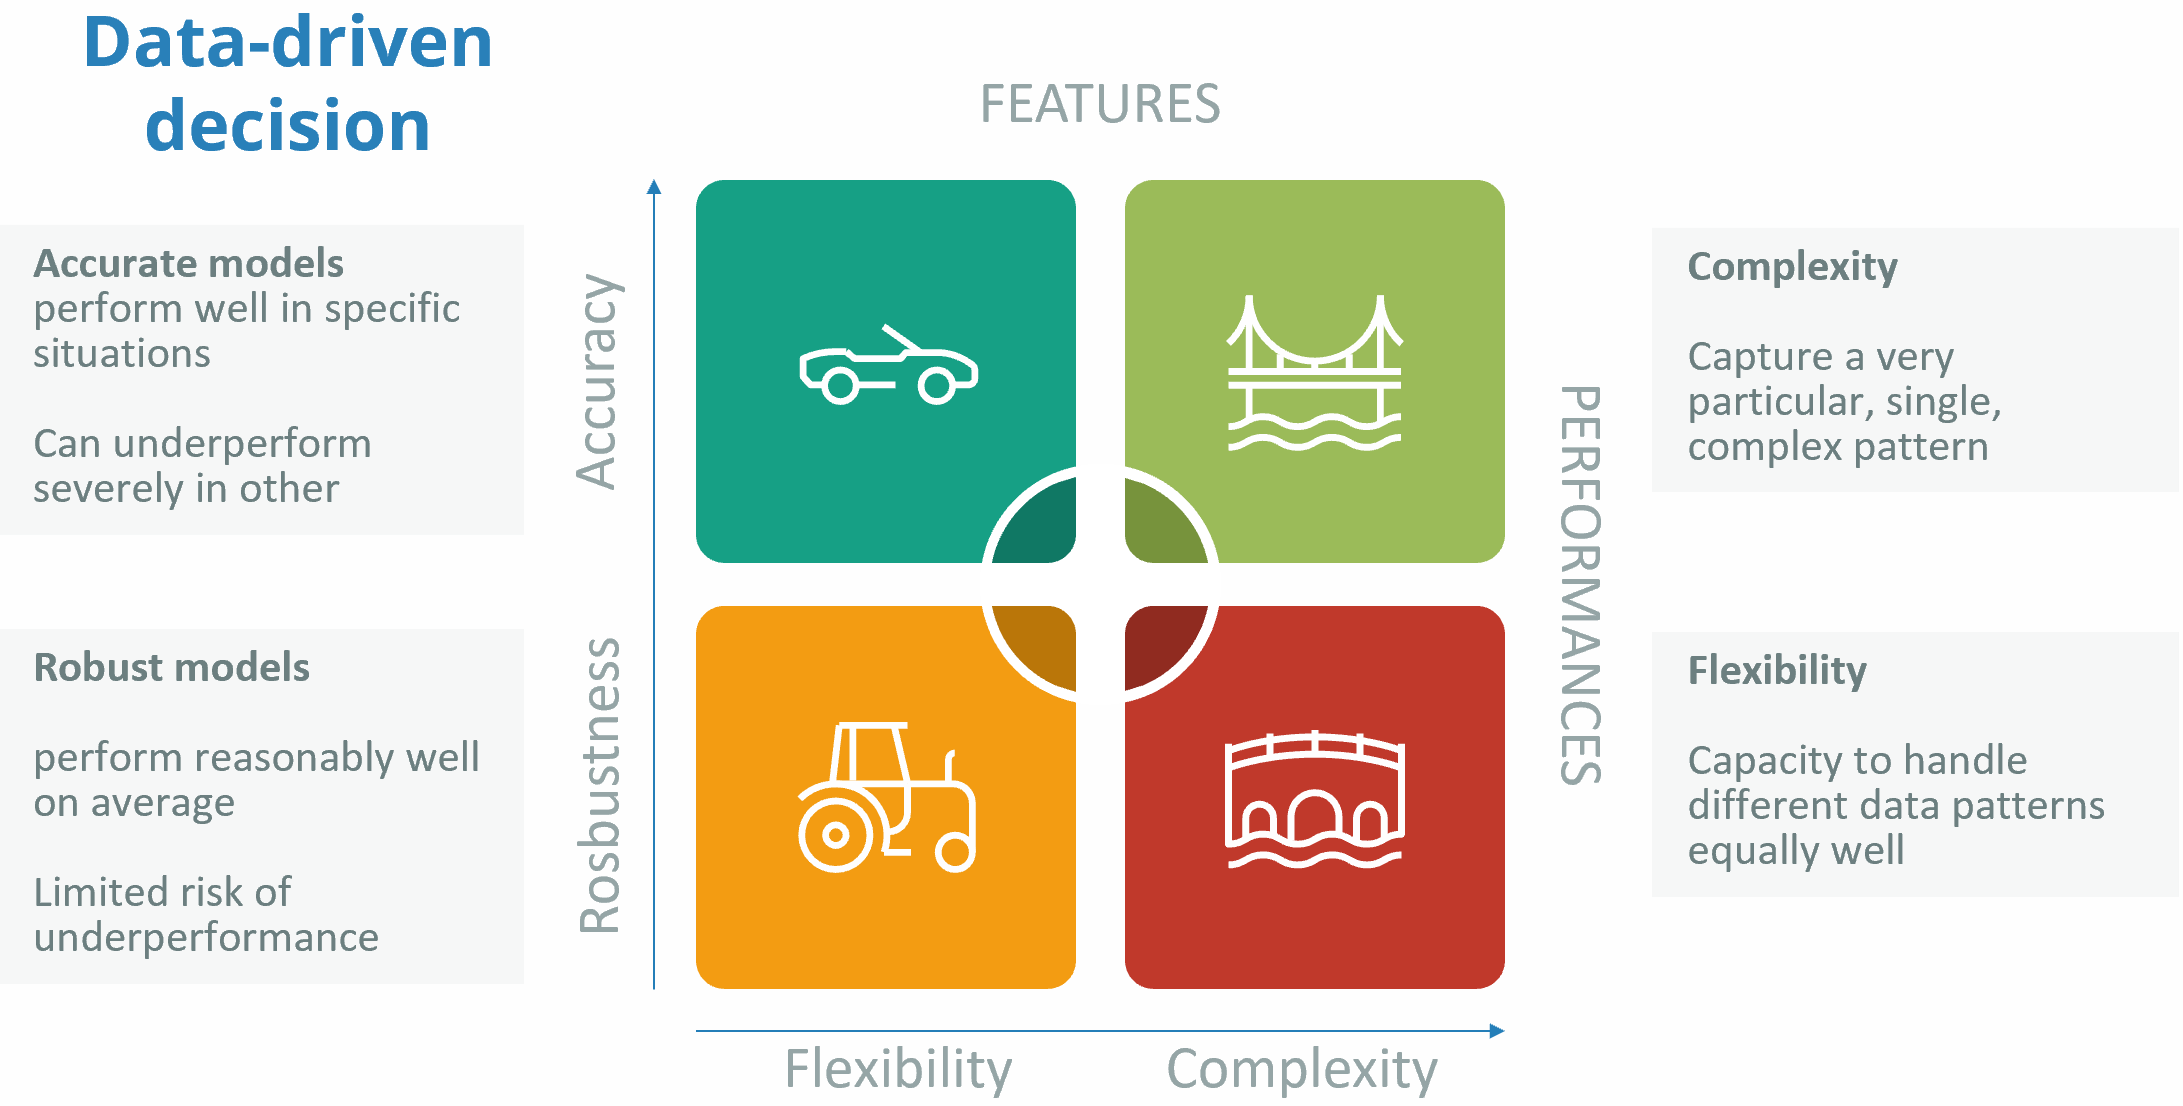
\includegraphics[width=0.85\paperwidth]{../static/course_2_img/statistical_tradeoffs.PNG}}
  \hspace*{15pt}\hbox{\scriptsize Credit:\thinspace{\scriptsize\itshape Author}}
\end{frame}


\begin{frame}
  \frametitle{Models Selection}
  \makebox[\linewidth]{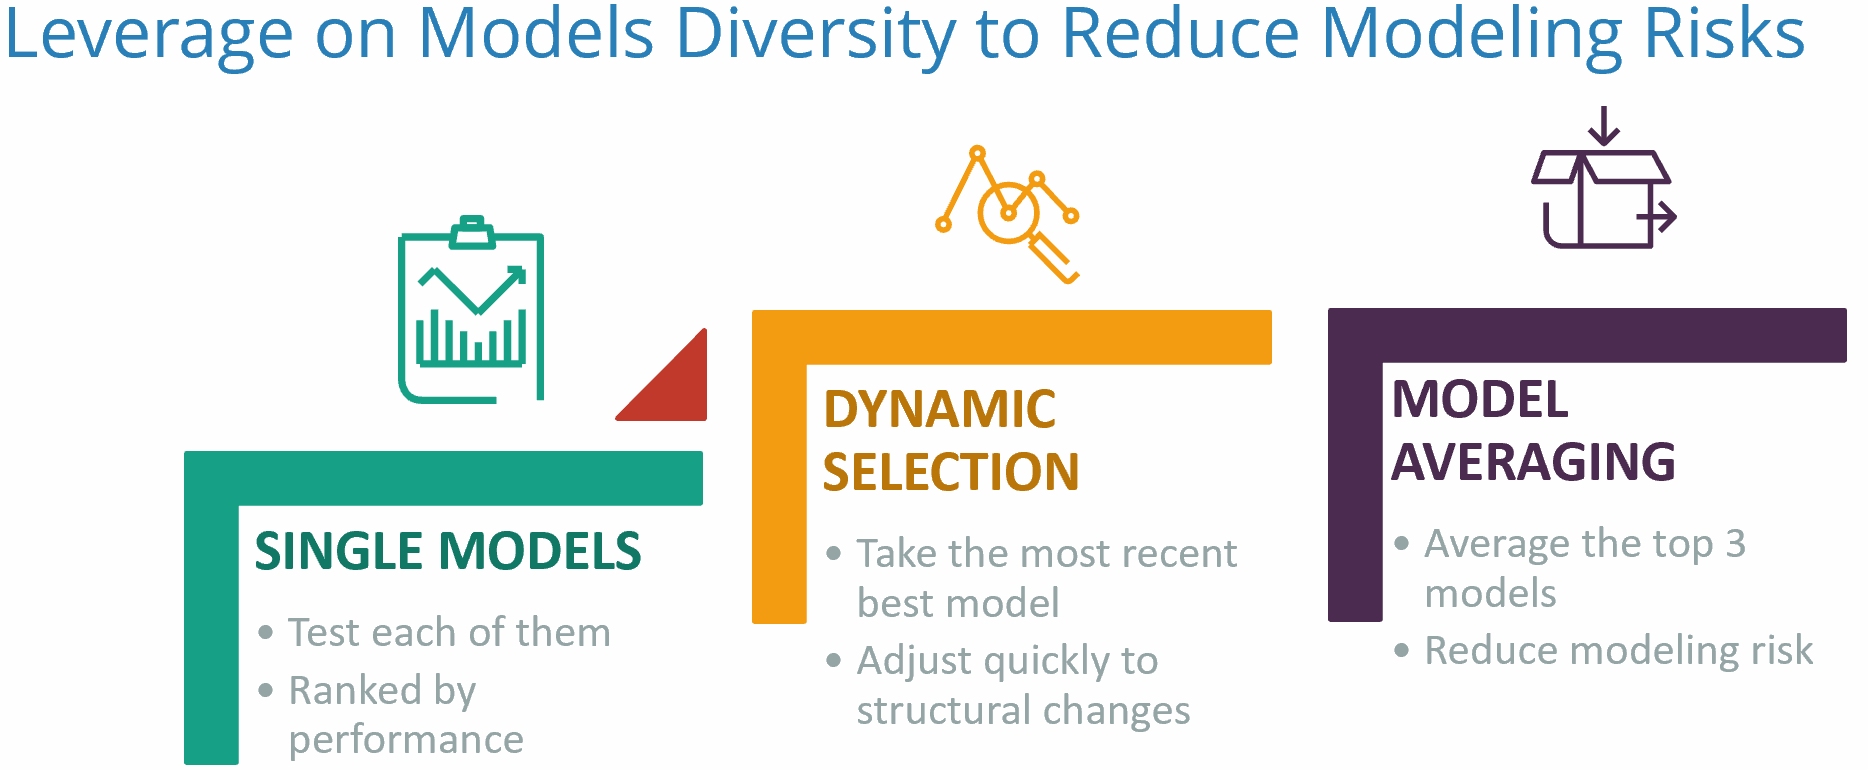
\includegraphics[width=0.85\paperwidth]{../static/course_2_img/model_selection.PNG}}
  \hspace*{15pt}\hbox{\scriptsize Credit:\thinspace{\scriptsize\itshape Author}}
\end{frame}


\begin{frame}
  \frametitle{Empirical Strategy}
  \makebox[\linewidth]{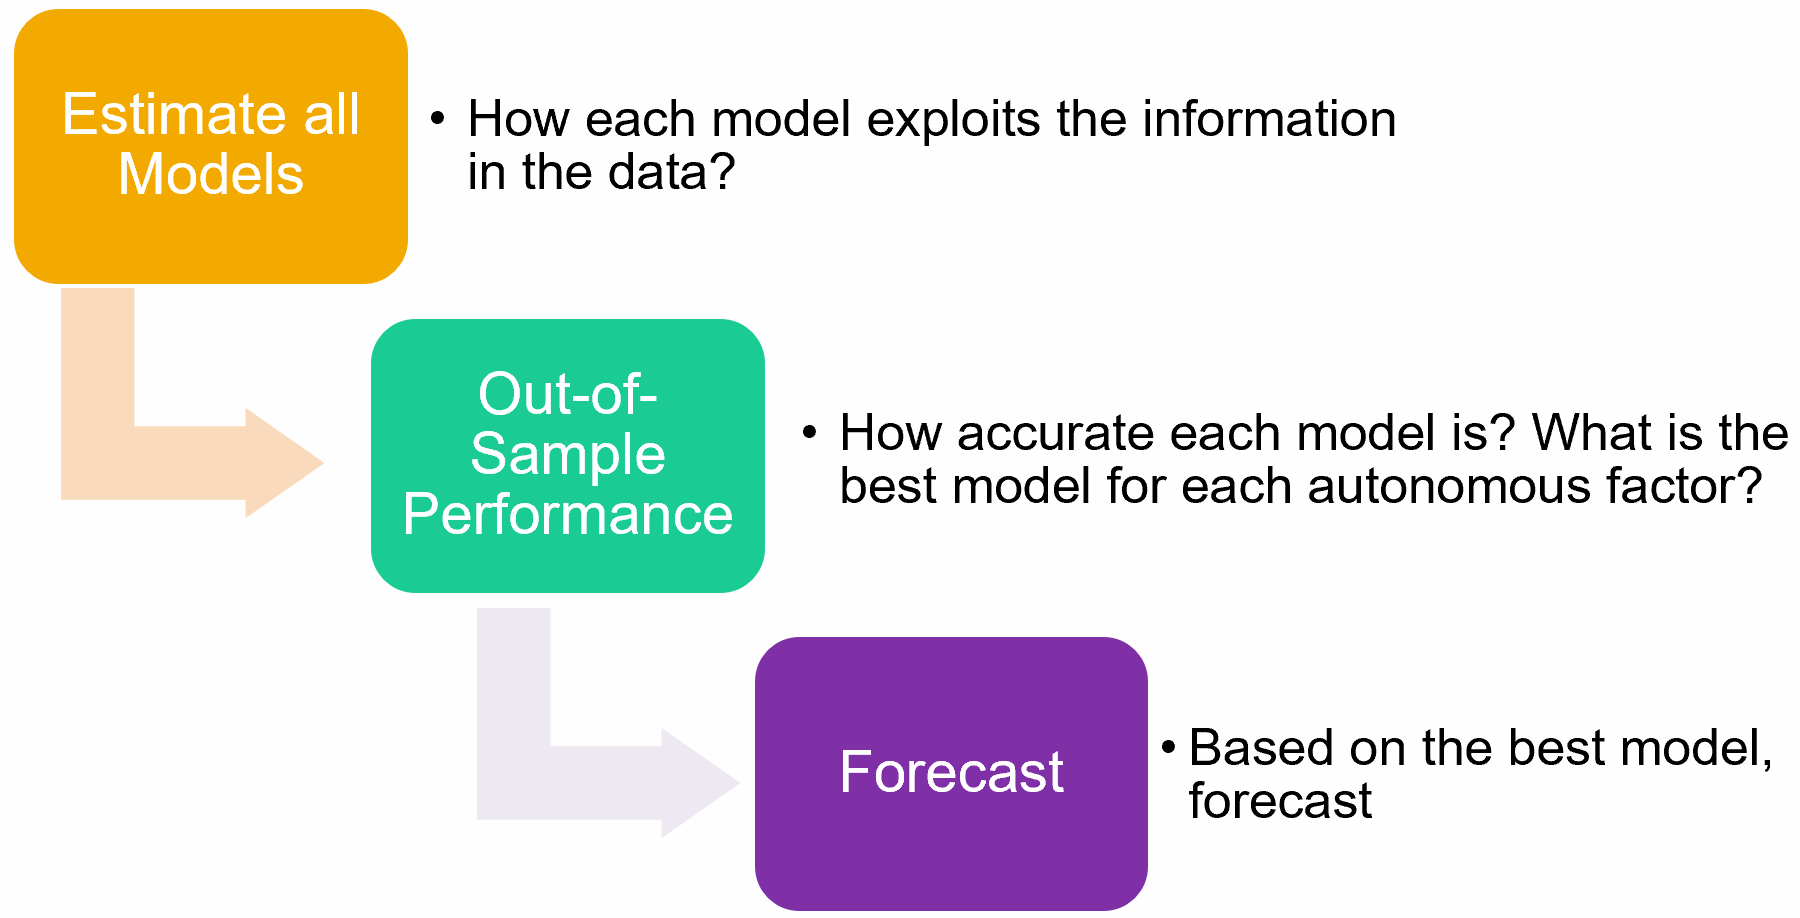
\includegraphics[width=0.85\paperwidth]{../static/course_2_img/empirical_strategy.PNG}}
  \hspace*{15pt}\hbox{\scriptsize Credit:\thinspace{\scriptsize\itshape Author}}
\end{frame}

\begin{frame}
  \frametitle{Underfit, Optimal, Overfit: Intuition}
  \makebox[\linewidth]{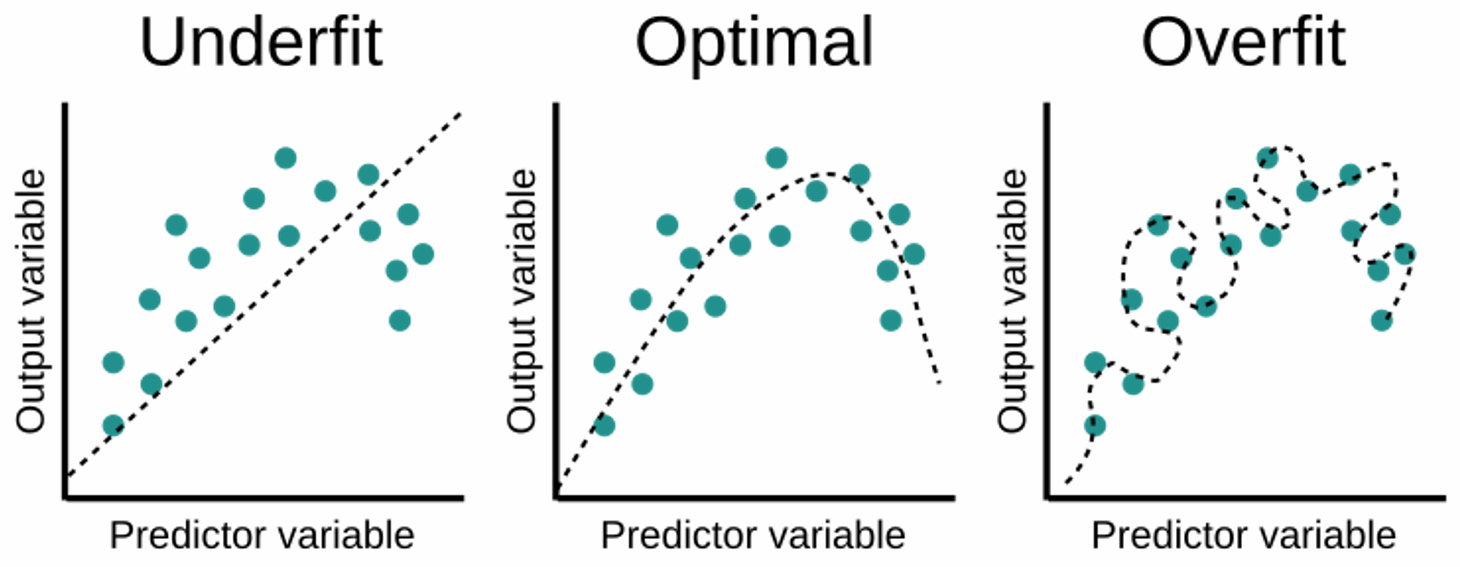
\includegraphics[width=0.95\paperwidth]{../static/course_3_img/overfit_underfit.PNG}}
  \hspace*{15pt}\hbox{\scriptsize Credit:\thinspace{\scriptsize\itshape towardsdatascience}}
\end{frame}


\begin{frame}
  \frametitle{Underfit, Optimal, Overfit and Model Complexity}
  \makebox[\linewidth]{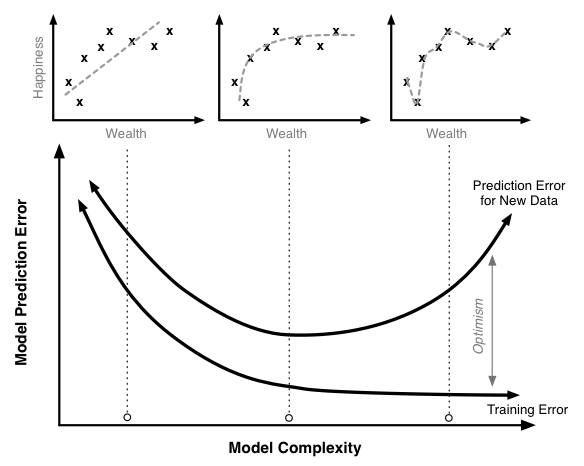
\includegraphics[width=0.85\paperwidth]{../static/course_2_img/prediction_error_complexity.png}}
  \hspace*{15pt}\hbox{\scriptsize Credit:\thinspace{\scriptsize\itshape Scott Fortmann-Roe}}
\end{frame}


\begin{frame}
  \frametitle{Out of Sample Concept}
  \makebox[\linewidth]{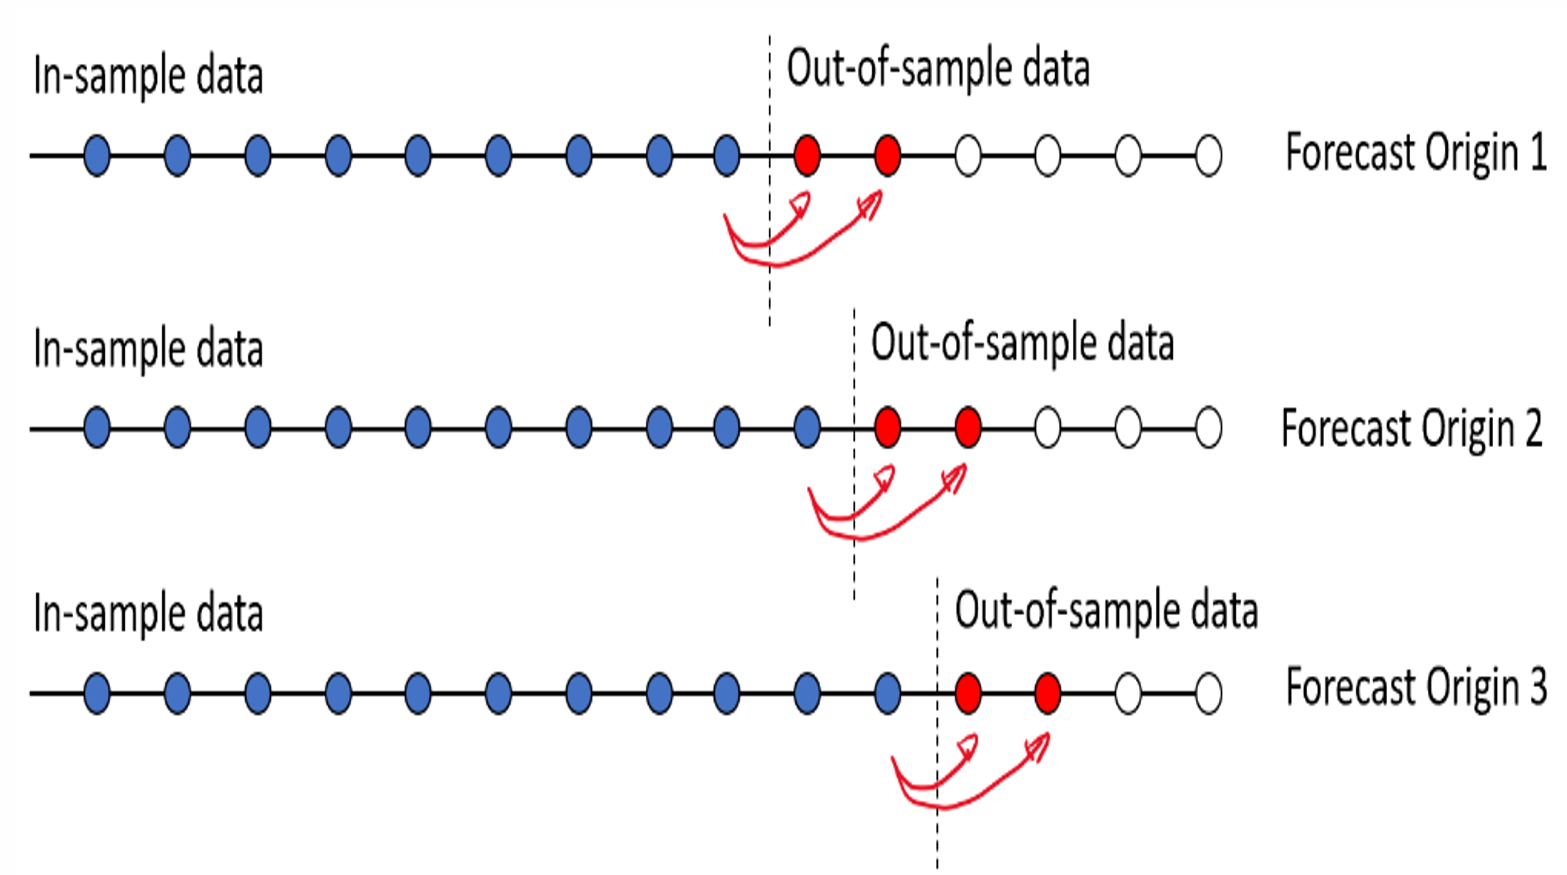
\includegraphics[width=0.75\paperwidth]{../static/course_2_img/out_of_sample_concept.PNG}}
  \hspace*{15pt}\hbox{\scriptsize Credit:\thinspace{\scriptsize\itshape Author}}
\end{frame}


\begin{frame}
  \frametitle{Out of Sample Example: Overfit}
  \makebox[\linewidth]{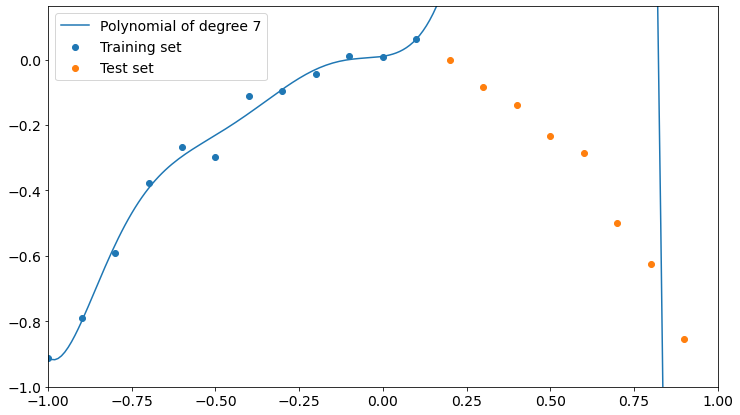
\includegraphics[width=0.85\paperwidth]{../static/course_2_img/overfit_poly_7.png}}
  \hspace*{15pt}\hbox{\scriptsize Credit:\thinspace{\scriptsize\itshape towardsdatascience.com/an-example-of-overfitting-and-how-to-avoid-it}}
\end{frame}


\begin{frame}
  \frametitle{Out of Sample Example: Correct Fit}
  \makebox[\linewidth]{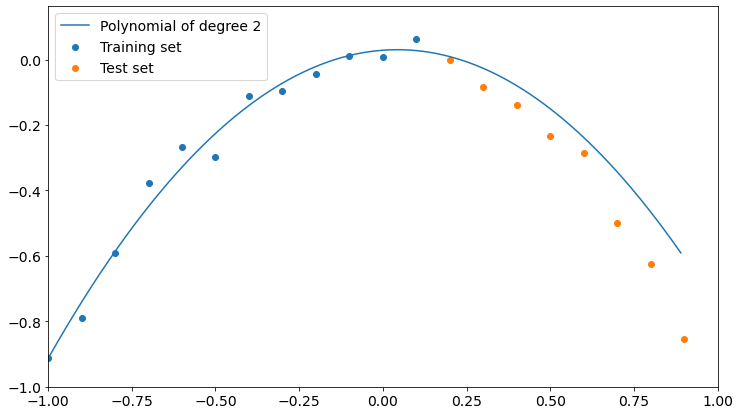
\includegraphics[width=0.85\paperwidth]{../static/course_2_img/fit_poly_2.png}}
  \hspace*{15pt}\hbox{\scriptsize Credit:\thinspace{\scriptsize\itshape towardsdatascience.com/an-example-of-overfitting-and-how-to-avoid-it}}
\end{frame}



\begin{frame}
  \frametitle{Operational Procedure}
  \makebox[\linewidth]{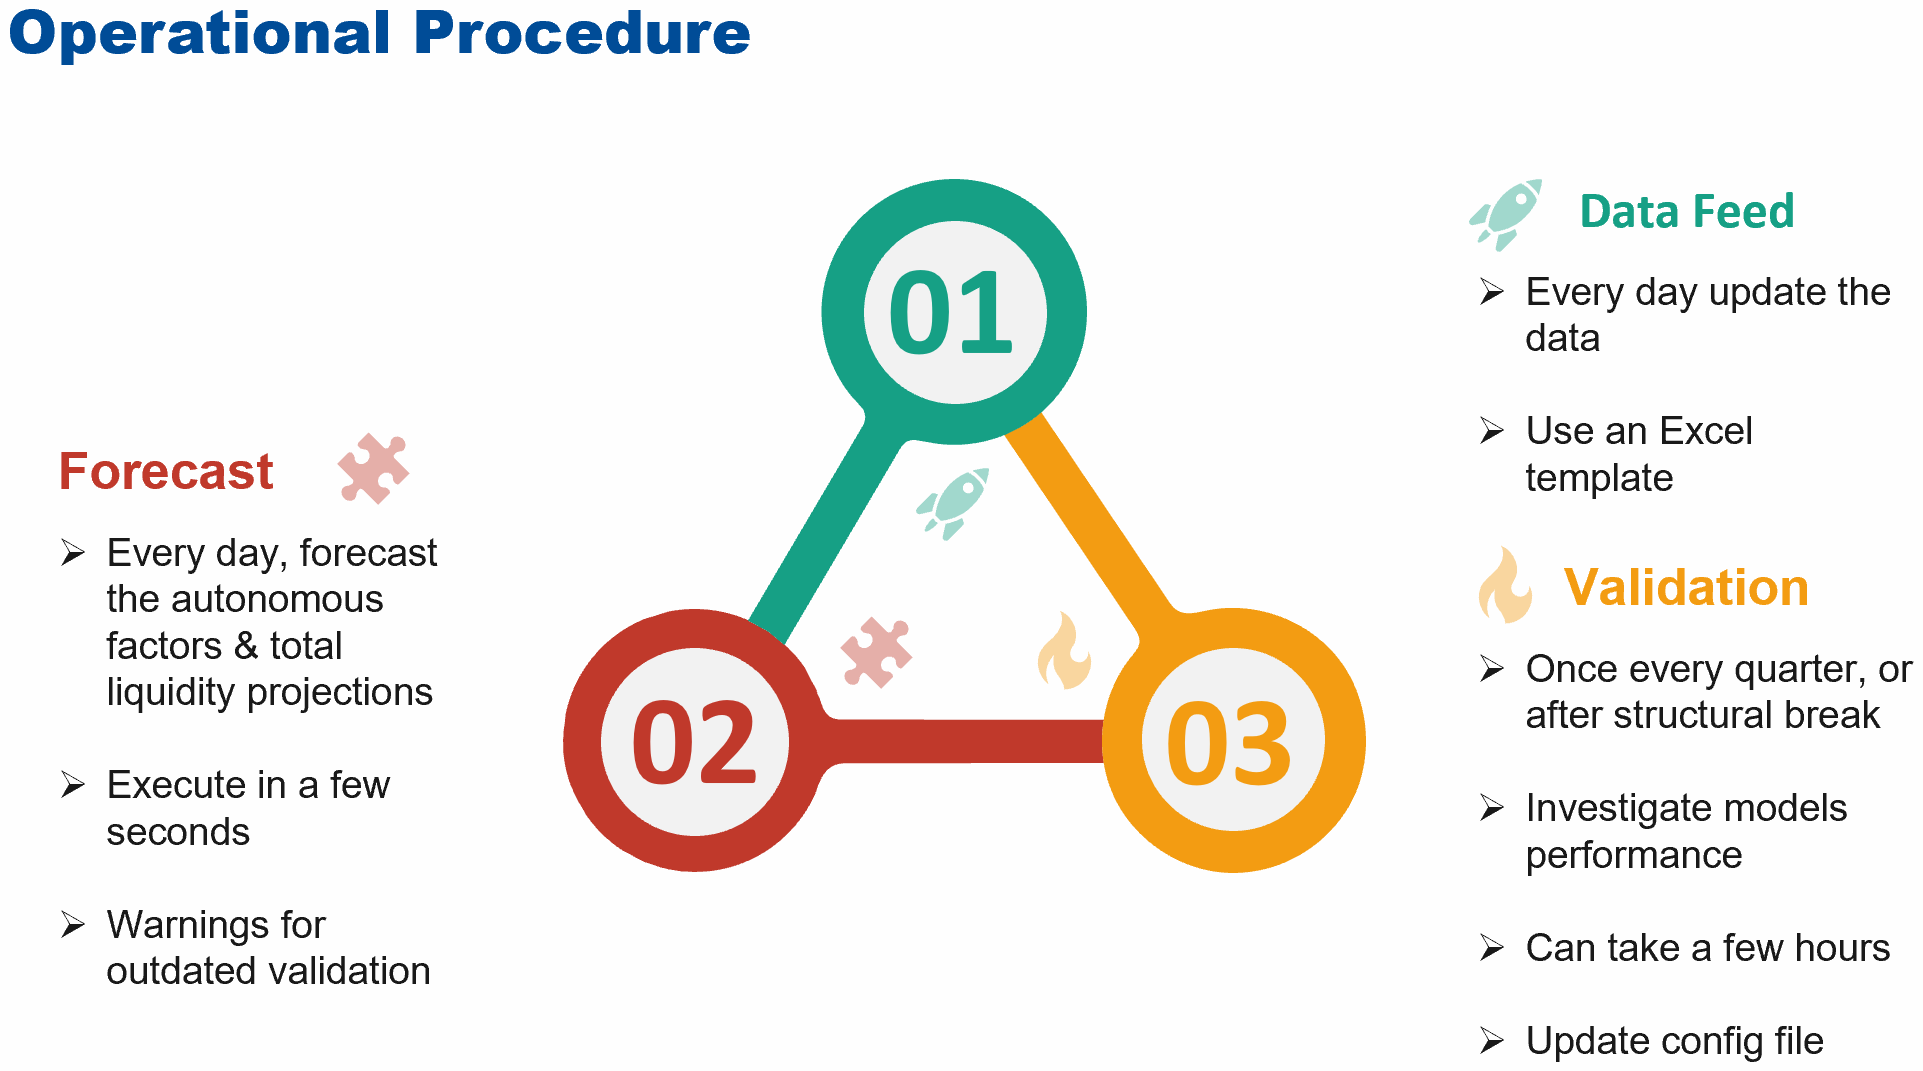
\includegraphics[width=0.85\paperwidth]{../static/course_2_img/operational_procedure.PNG}}
  \hspace*{15pt}\hbox{\scriptsize Credit:\thinspace{\scriptsize\itshape Author}}
\end{frame}



\begin{frame}
  \frametitle{Software Infrastructure}
    \makebox[\linewidth]{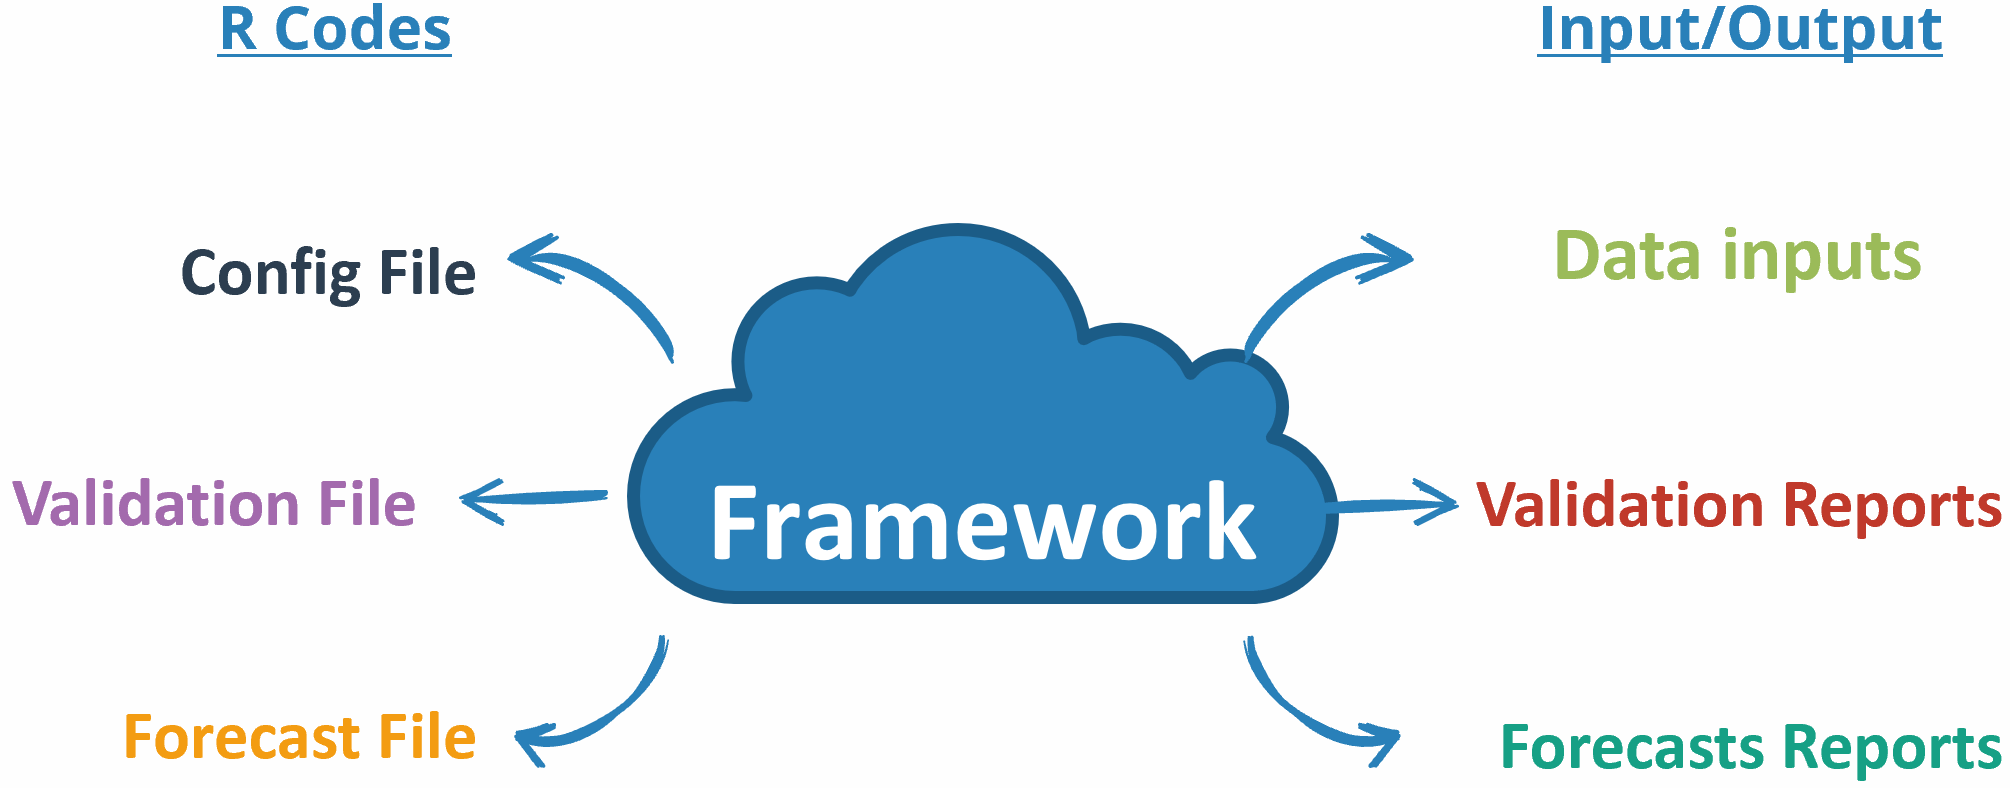
\includegraphics[width=0.85\paperwidth]{../static/course_2_img/software_infrastructure.PNG}}
  \hspace*{15pt}\hbox{\scriptsize Credit:\thinspace{\scriptsize\itshape Author}}

\end{frame}

\begin{frame}
    \frametitle{What Constitutes a Good Estimator?}
    The idea is to study the properties of the \textbf{sampling distribution} of the estimator $\hat{\theta}$, and especially its moments, such as:\\

    \medskip

    \begin{wideitemize}
    \item $\mathbb{E}[\hat{\theta}]$ for the biais: the difference between the true value and the point estimate
    \item $\mathbb{V}[\hat{\theta}]$ for the precision: the variance of the estimator
    \item $\mathbb{S}[\hat{\theta}]$ for the symmetry
    \item $\mathbb{K}[\hat{\theta}]$ for the tail-risks  
    \item etc.
    \end{wideitemize}
  \end{frame}


  \begin{frame}
    \frametitle{Estimators Properties}
    Estimators are compared on the basis of a variety of attributes

    \begin{wideenumerate}
      \item \textbf{Finite sample properties} (or finite sample distributions) investigate how the estimator behave when the observational sample is relatively limited (a few hundreds to a few thousands of observations max)
      \item However, these properties rely on a distributional assumption (usually normality or gaussianity), that may be difficult to test. 
      \item When the normality assumption is no longer valid (and the finite sample distribution is unknown), estimators are evaluated on the basis on their \textbf{large sample}, or \textbf{asymptotic properties}
    \end{wideenumerate}    
  \end{frame}


  \begin{frame}
    \frametitle{Finite Sample Theorem}
    \begin{block}{Theorem: Finite Sample Distributions}
        If we assume that, with a sample of size $T$, generated from a stochastic process with i.i.d random variables $X_1, X_2, \dots, X_T$  with $X_{t} \sim \mathcal{N}(\mu, \sigma^2)$, then the estimators of the sample mean $\hat{\mu_T}$ and the estimator of the sample variance/population variance $(T-1) \frac{\hat{\sigma^2_T}}{\sigma^2}$ have a \textbf{finite sample distribution}

        \begin{equation*}
          \hat{\mu_T} = \mathcal{N}\left(\mu, \frac{\sigma^2}{T} \right) \qquad \forall \ T \ \in \ \mathbb{N}
        \end{equation*}


        \begin{equation*}
          \frac{T-1}{\sigma^2} \hat{\sigma^2} \sim \chi^{2} (T-1) \qquad \forall T \ \geq \ 2
        \end{equation*}
        
      \end{block}
\end{frame}


\begin{frame}
      \begin{exampleblock}{Example: Finite Sample Distribution}
        Under the Gaussianity assumption, with a sample size of $T = 10$, then:
        \begin{equation*}
          \hat{\mu} \sim \mathcal{N}\left( \mu, \frac{\sigma^2}{10} \right) \qquad 9 \times \frac{\hat{\sigma^2_T}}{\sigma^2} \sim \chi^2(9)
        \end{equation*}        
      \end{exampleblock}
      
  \end{frame}
  

  \begin{frame}
    \frametitle{Difficulties with Finite Sample Inference}
    In most cases, it is impossible to derive the \textbf{exact/finite sample distribution} for the estimator (or any transformation of the estimator).

    \begin{wideenumerate}
    \item In some cases, the exact distribution of $\{ X1, X2, \dots, X_T\}$ is known, but the estimator function $S()$ (also called the "statistics") is too complicated
      \begin{equation*}
        \hat{\theta} = S(X_1, X_2, \dots, X_T) \sim ??? \qquad \forall \ T \ \in \mathbb{N}
      \end{equation*}

      \item In most cases, the distribution of the stochastic process $\{X1, X2, \dots, X_T\}$ is unknown

      \begin{equation*}
        \hat{\theta} = S(X_1, X_2, \dots, X_T) \sim ??? \qquad \forall \ T \ \in \mathbb{N}
      \end{equation*}        
    \end{wideenumerate}
    
  \end{frame}
  


  \begin{frame}
    \frametitle{Asymptotic Properties}

    What is the behavior of the estimator $\hat{\theta_T}$ when the sample size $T$ tends to infinity?

    \begin{block}{Definition: Asymptotic Theory}
      \textbf{Asymptotic} or \textbf{large sample theory} consists in the study of the distribution of the estimator when the sample size is sufficiently large (usually, more than 10k)
    \end{block}

    The asymptotic theory is fundamentally based on the notion of \textbf{convergence}
    
  \end{frame}
  

  \begin{frame}
    \frametitle{Convergence in Probability}
    There are many types of convergence, but typically applied statisticians are interested in:
   
    \begin{enumerate}
      \item Convergence in probability
      \item Convergence in distribution
    \end{enumerate}

    \begin{itemize}
\item  \textbf{Convergence in probability} (also called "mean squared convergence" or "almost sure convergence")

  \begin{equation*}
    \hat{\theta_T} \ \overset{p}{\to} \ \theta \qquad \text{for} \ \theta \ \in \ \mathbb{R}
  \end{equation*}

\item Technically, for a stochastic process ${\theta_T}_{-\infty}^ {+\infty}$
  \begin{equation*}
  \hat{\theta_T} \ \overset{p}{\to} \theta \quad \Leftrightarrow \quad \text{lim}_{T \to +\infty} \mathbb{P} \left[ |\theta_T - \theta| > \epsilon \right] \ = \ 0 
  \end{equation*}
    
\item The convergence in probability is used to derive the \textbf{consistency property} of estimators
    \end{itemize}
    
  \end{frame}


  \begin{frame}
    \frametitle{Illustration: Distribution in Probability}
    
    \begin{equation*}
\hat{X_T} \ \overset{p}{\to} c \ \text{if} \ \Leftrightarrow \quad \text{lim}_{T \to +\infty} \mathbb{P} \left[ |X_T - c| > \epsilon \right] \ = \ 0      
    \end{equation*}
    
     \makebox[\linewidth]{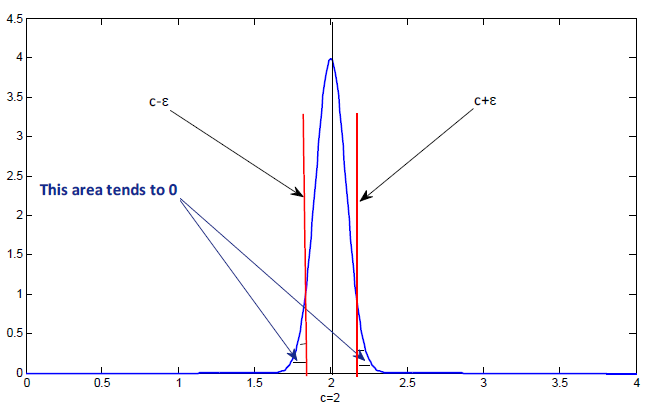
\includegraphics[width=0.7\paperwidth]{../static/course_1_img/distribution_in_proba.PNG}}
    
  \end{frame}


  \begin{frame}
    \frametitle{Interpretation}
    \begin{wideenumerate}
    \item The distribution of the sample moments is highly concentrated around the true value (unknown) of the population moment when the sample size $T$ tends to infinity
    \item In other words, over a very large sample of data (for instance, hundred of thousands of observations) the \textbf{moments estimated in the sample} are then very "close" to the true value of \textbf{the moments in the population}
    \end{wideenumerate}
  \end{frame}
  

  \begin{frame}
    \frametitle{Consistent Estimator}
    \begin{alertblock}{Definition}
      An estimator is consistent if it converges in probability towards the true value

      \begin{equation*}
        \hat{\theta}_T \ \overset{p}{\to} \theta \ \text{if} \ \Leftrightarrow \quad \text{lim}_{T \to +\infty} \mathbb{P} \left[ |\theta_T - c| > \epsilon \right] \ = \ 0      
      \end{equation*}
    \end{alertblock}

    \begin{wideitemize}
      \item Consistency can be slow or fast: how many observations do we need to be "reasonably" close to the true value?
      \item Estimators can be inconsistent if they suffer from endogeneity, non-random observational noise, simultaneity bias, etc.  
    \end{wideitemize}
    
  \end{frame}


  \begin{frame}
    \frametitle{Example of Inconsistency: The Simpson Paradox}
    \makebox[\linewidth]{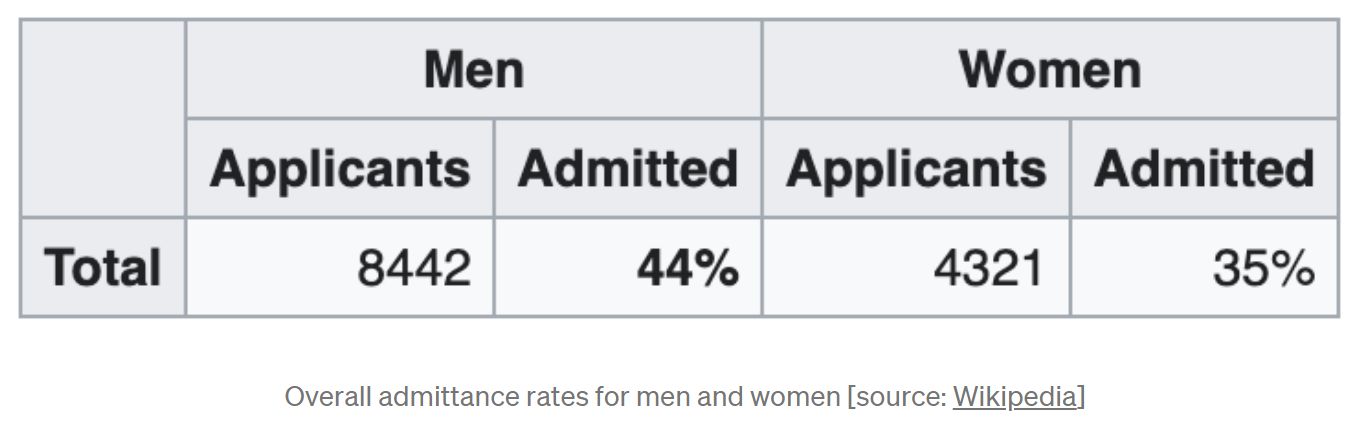
\includegraphics[height=0.25\paperheight]{../static/course_1_img/simpson_1.PNG}}
    \makebox[\linewidth]{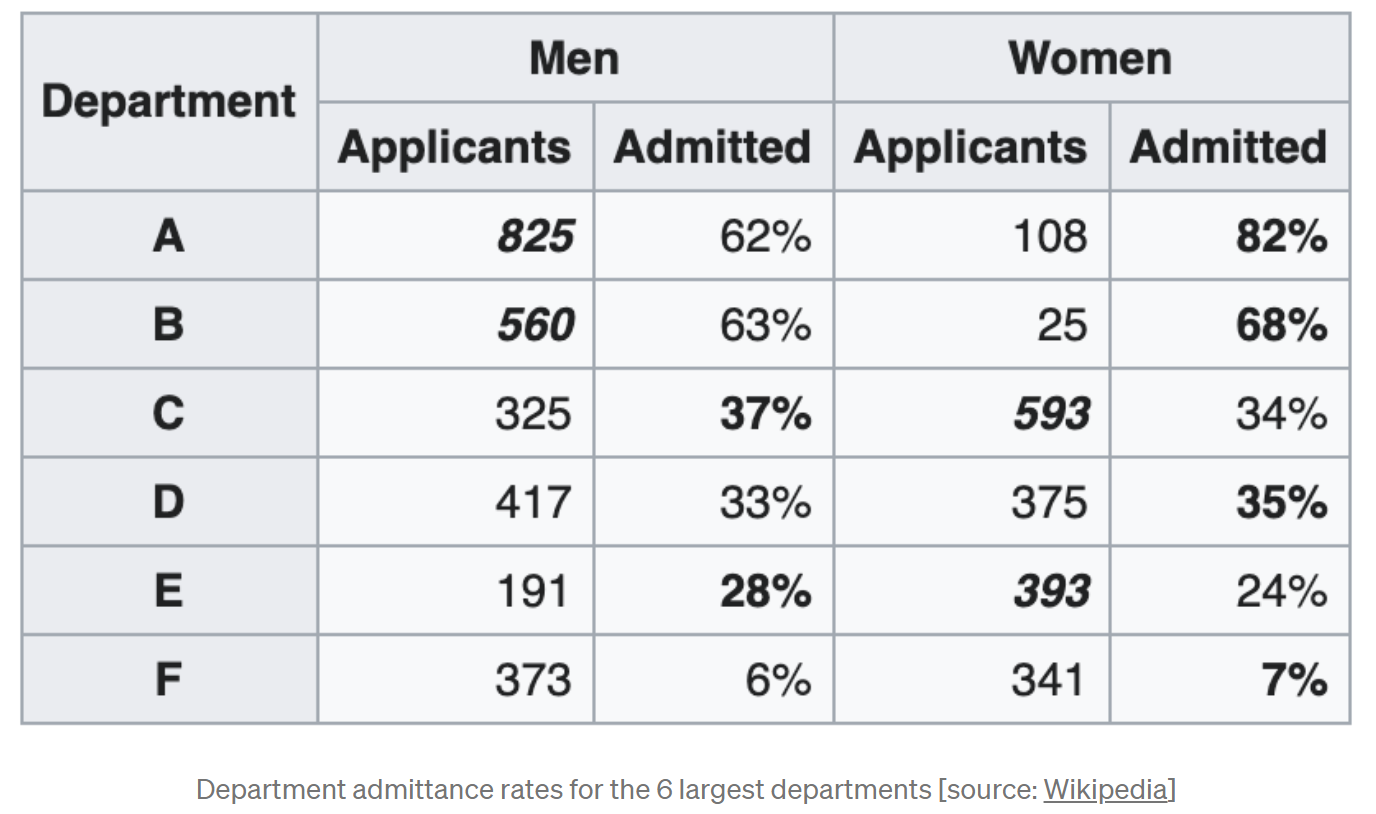
\includegraphics[height=0.4\paperheight]{../static/course_1_img/simpson_2.PNG}}
      \hspace*{15pt}\hbox{\scriptsize Credit:\thinspace{\scriptsize\itshape towardsdatascience.com/what-is-simpsons-paradox-4a53cd4e9ee2}}    
  \end{frame}

  
  \begin{frame}
    \frametitle{Endogeneity due to Omitted Variable: Simpson Paradox}
      \makebox[\linewidth]{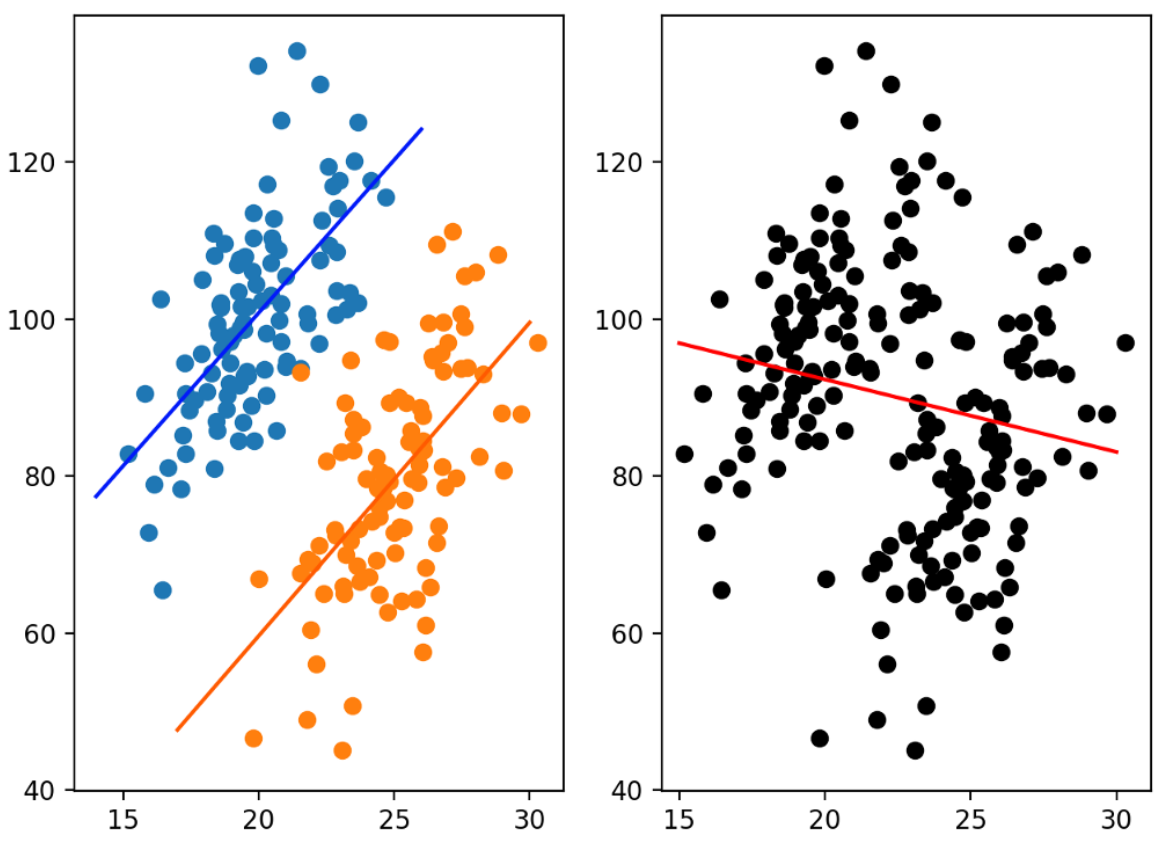
\includegraphics[width=0.8\paperwidth]{../static/course_1_img/simpson_paradox.PNG}}
      \hspace*{15pt}\hbox{\scriptsize Credit:\thinspace{\scriptsize\itshape towardsdatascience.com/what-is-simpsons-paradox-4a53cd4e9ee2}}    
  \end{frame}

  
  \begin{frame}
    \frametitle{Biased and Unbiased Estimator}

      \begin{wideitemize}
        \item We are interesting in recovering the true parameter $\theta$ of a DGP ${y_t}_{t \ \in \ \mathbb{Z}} = \mathcal{D}[Y, \theta]$ 
        \item We have an estimator $\hat{\theta}$
      \end{wideitemize}

      \begin{alertblock}{Definition: Estimator Bias}
        
        \begin{equation*}
          \text{Bias}(\hat{\theta}) = E_Y[\hat{\theta}] - \theta = E_Y[\hat{\theta} - \theta]
        \end{equation*}        
    \end{alertblock}

    \begin{block}{Difference between Consistency and Bias}
    \begin{wideitemize}
      \item Note that an estimator can be consistent but biased (e.g. for the mean $\frac{1}{n}\sum x_i + \frac{1}{n}$)
      \item Likewise, an estimator can be inconsistent and unbiased (e.g $\frac{1}{n}\sum x_i + \text{sin}(n)$)
    \end{wideitemize}
      
    \end{block}
    
    
  \end{frame}


  \begin{frame}
    \frametitle{Consistency vs. Bias}
    \makebox[\linewidth]{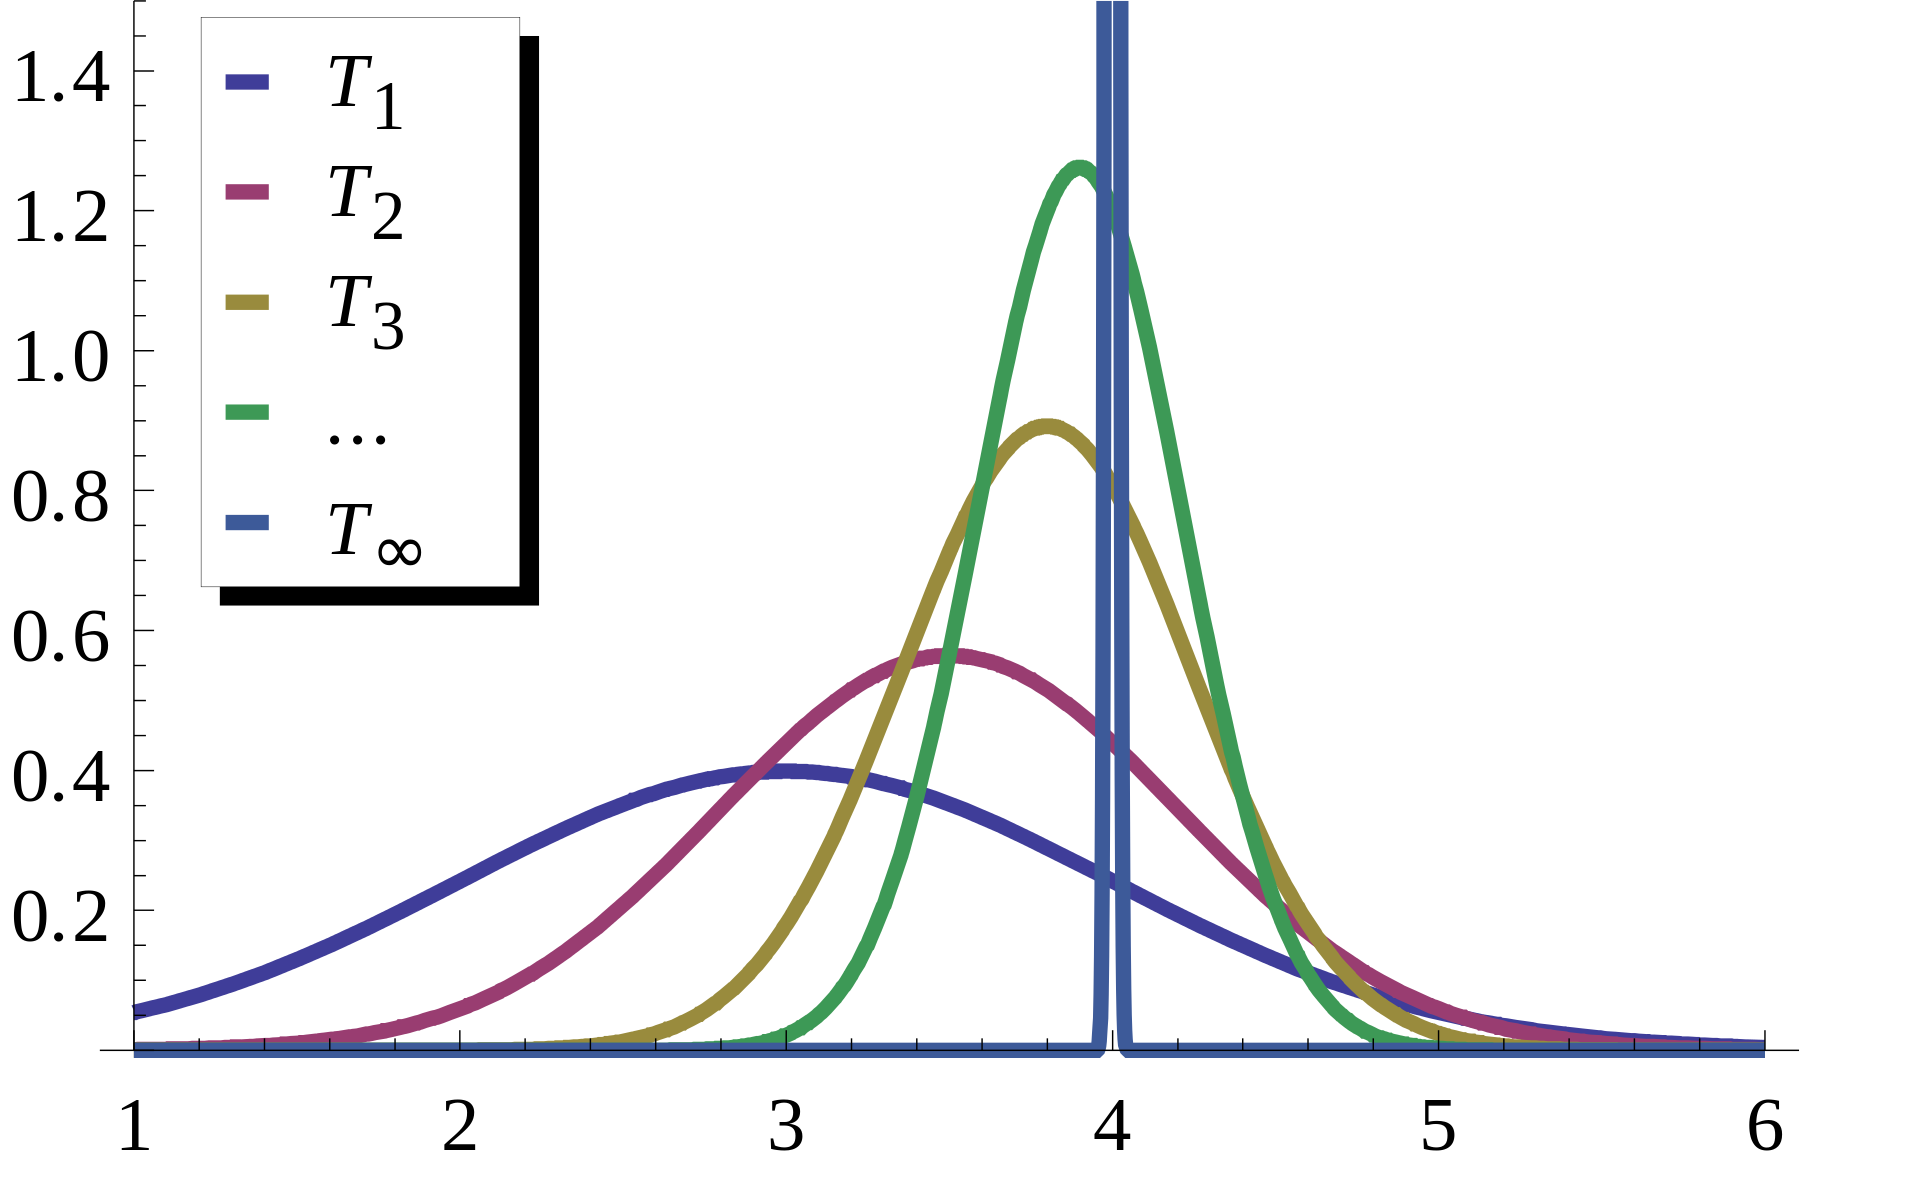
\includegraphics[width=0.85\paperwidth]{../static/course_1_img/consistency.PNG}}
    \hspace*{15pt}\hbox{\scriptsize Source:\thinspace{\scriptsize\itshape Wikipedia}}    
  \end{frame}
  
  
  \begin{frame}
    \frametitle{For information: Convergence in Distribution}

    \begin{itemize}
\item  \textbf{Convergence in distribution} is interested in the distribution of the bias (the distance between the estimator and the true value)

  \begin{equation*}
    \sqrt{T} \left(\hat{\theta_T} - \theta_0 \right) \ \sim \ \mathcal{N}(\mu_., \sigma_.) \qquad \mathcal{N} \ \text{is the most common} 
  \end{equation*}

\item Technically, for a stochastic process ${X_T}_{-\infty}^ {+\infty}$, with a cdf $F_T(.)$; $X_T$ is said to \textbf{converge in distribution} to a random variable $X$ if:
  \begin{equation*}
X_t \ \overset{d}{\to} \ X \quad \Leftrightarrow \quad  F_T(x) = F(x) \qquad \ \forall \ x \ \in \ \mathbb{R}
  \end{equation*}
    
\item The convergence in distribution is used to derive the \textbf{asymptotic distribution} of the estimators and to make \textbf{inference} (tests) about the true value of the parameters

    \end{itemize}    
  \end{frame}


  \begin{frame}
    \frametitle{Bias, Variance and Mean-Squared Error}

    \begin{block}{Mean Squared Error of an Estimator}
      \begin{equation*}
        \text{MSE}(\hat{\theta}) = \mathbb{E}\left[ (\hat{\theta} - \theta)^2 \right]
      \end{equation*}
    \end{block}


    \begin{alertblock}{$\text{MSE} = \text{Bias}^2 + \text{Variance}$}
      \begin{equation*}
       \text{MSE}(\hat{\theta}) = \underbrace{\left(\mathbb{E}(\hat{\theta}) -\theta \right)^2}_{\text{Bias}^2(\hat{\theta})} + \underbrace{\mathbb{E}\left[(\hat{\theta} - \mathbb{E}[\hat{\theta}]) \right]}_{\mathbb{V}(\hat{\theta})}
      \end{equation*}
    \end{alertblock}
    
  \end{frame}


  \begin{frame}
    \frametitle{Bias Variance Tradeoff: Intuition}
      \makebox[\linewidth]{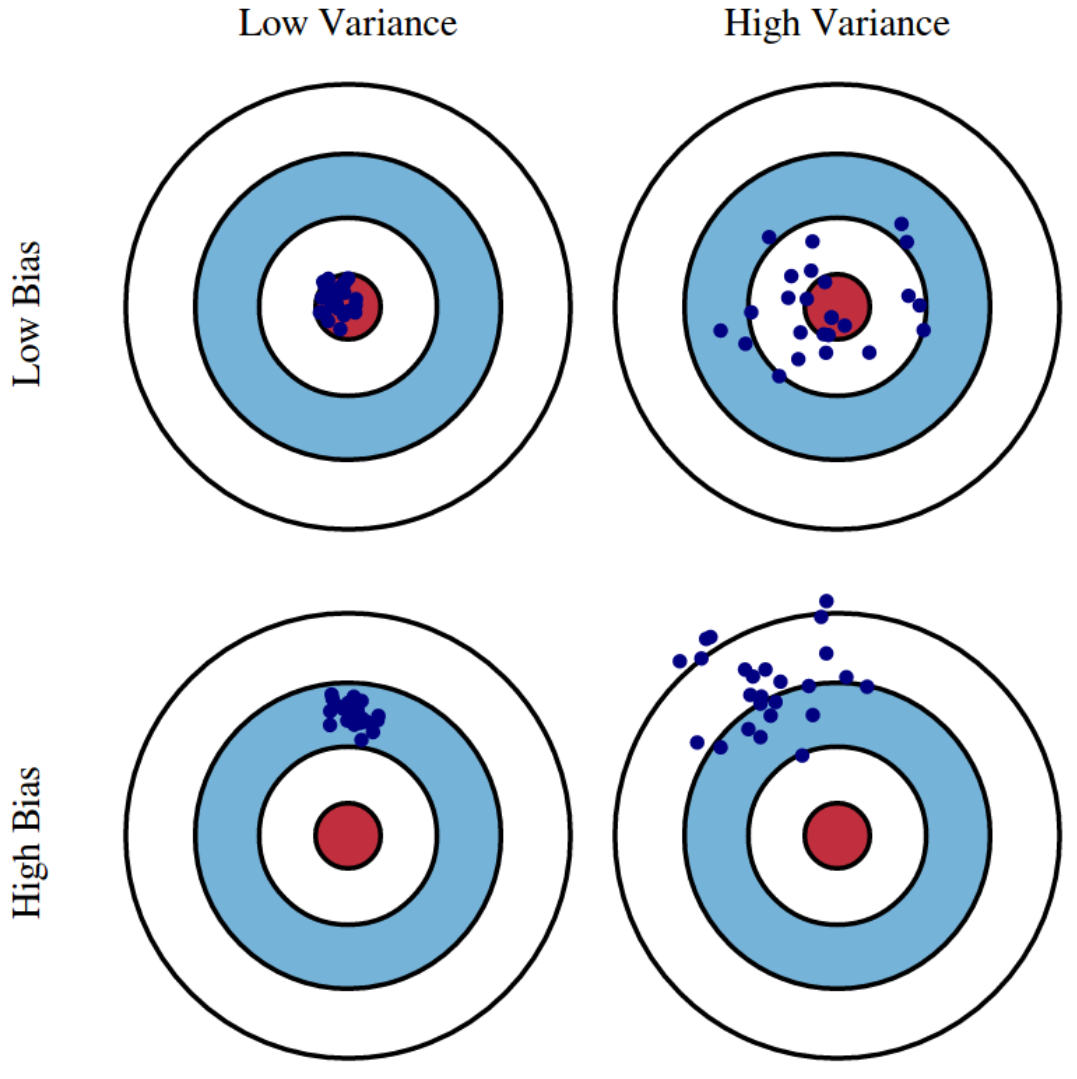
\includegraphics[height=0.8\paperheight]{../static/course_1_img/bias_variance_tradeoff.PNG}}
      \hspace*{15pt}\hbox{\scriptsize Credit:\thinspace{\scriptsize\itshape www.cs.cornell.edu/courses/cs4780/2018fa/lectures}}

  \end{frame}


  \begin{frame}
    \frametitle{Would you Choose $\hat{beta}_1$ or $\hat{beta}_2$?}
      \makebox[\linewidth]{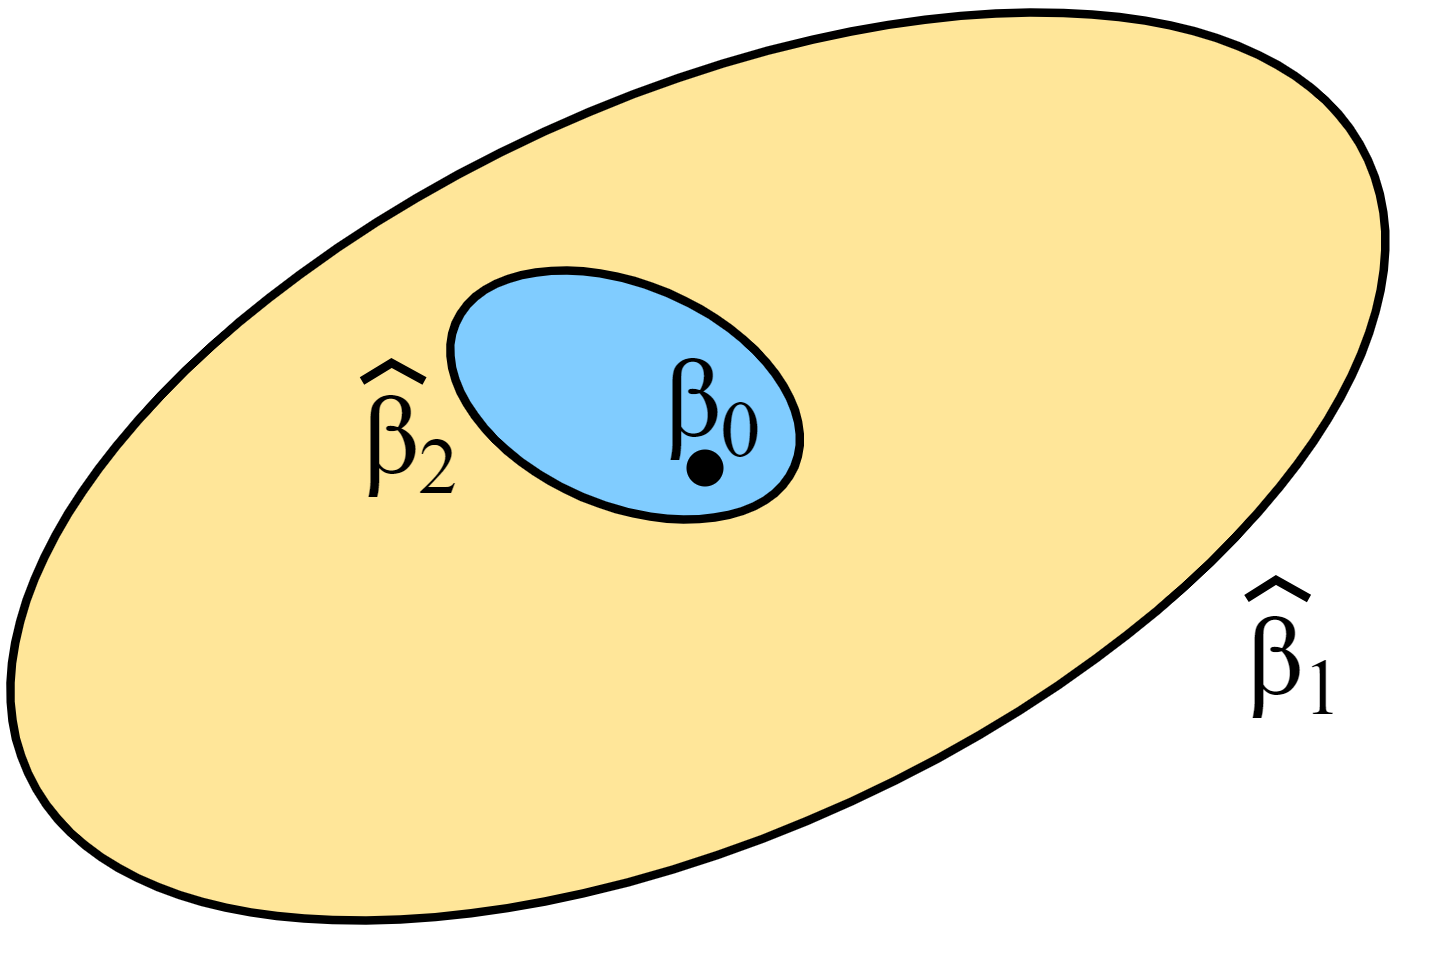
\includegraphics[height=0.7\paperheight]{../static/course_1_img/bias_variance_circle.PNG}}
      \hspace*{15pt}\hbox{\scriptsize Credit:\thinspace{\scriptsize\itshape www.cs.cornell.edu/courses/cs4780/2018fa/lectures}}

  \end{frame}

  
  
  \begin{frame}
    \frametitle{Bias Variance Tradeoff}

    \begin{wideitemize}
    \item Bias–variance tradeoff: property of a model that the variance of the parameter estimated across samples can be reduced by increasing the bias in the estimated parameters
      
    \item The bias error is an error from erroneous assumptions in the learning algorithm.
      \begin{itemize}
      \item High bias can cause an algorithm to miss the relevant relations between features and target outputs (underfitting)
      \end{itemize}

        
    \item The variance is an error from sensitivity to small fluctuations in the training set.
      \begin{itemize}
      \item High variance may result from an algorithm modeling the random noise in the training data (overfitting)
      \end{itemize}             
    \end{wideitemize}
      
  \end{frame}

  
\begin{frame}
  \frametitle{Underfit, Optimal, Overfit: Intuition}
  \makebox[\linewidth]{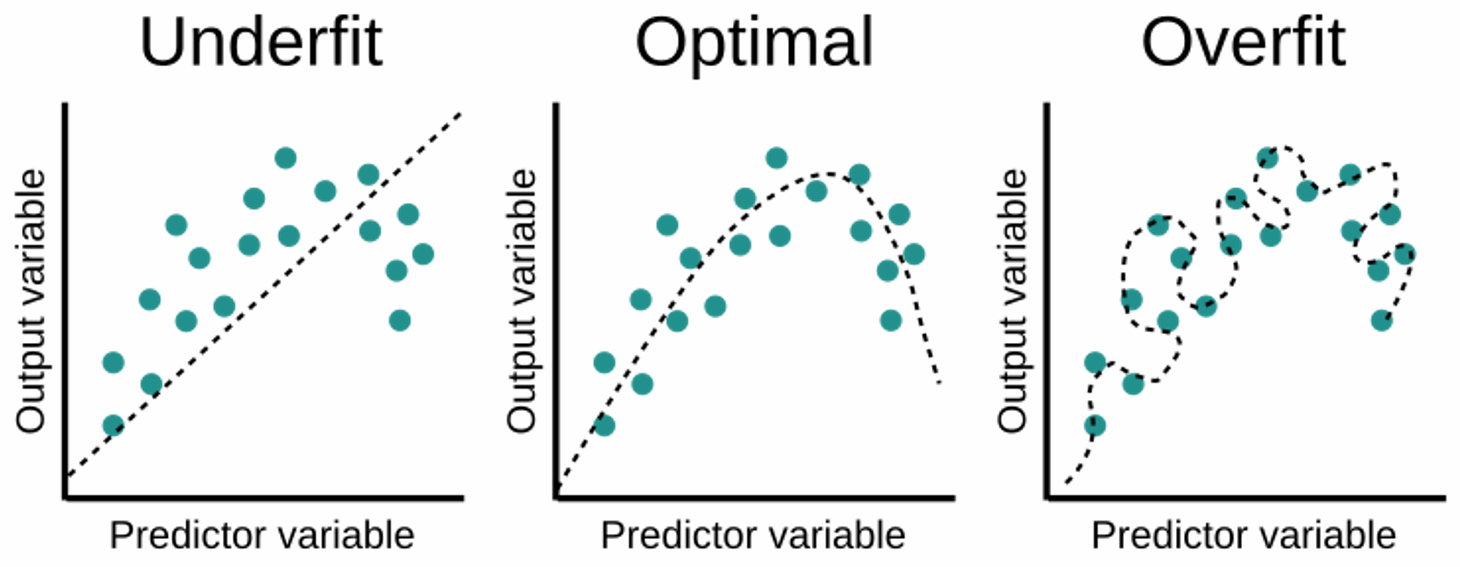
\includegraphics[width=0.95\paperwidth]{../static/course_3_img/overfit_underfit.PNG}}
  \hspace*{15pt}\hbox{\scriptsize Credit:\thinspace{\scriptsize\itshape towardsdatascience}}
\end{frame}

 \section{Q \& A}

\begin{frame}
  \frametitle{Question 1}
  
  \textbf{What are the benefits of accurate liquidity forecasting for central banks operations? Multiple answers possible:}\\

  \bigskip

  \begin{wideenumerate}
    \item Reduce inflation
    \item Better calibrate the operations
    \item Reduce the interbank interest rate volatility 
    \item Stabilize the exchange rate
    \item Support the interbank market development
  \end{wideenumerate}
  
\end{frame}



\begin{frame}
  \frametitle{Question 2}
  \textbf{Which strategy is valid to reduce the risk of being reliant of a single model (modeling risks)}? Multiple answers possible:\\
  \bigskip

  \begin{wideenumerate}
  \item Model averaging
  \item Use large data sample 
  \item Remove outliers
  \item Dynamic model selection
  \item Complement the results with expert judgment
   
  \end{wideenumerate}
  
\end{frame}



\begin{frame}
  \frametitle{Question 3}

  \textbf{Why is it more appropriate to evaluate the performance of models out-of-sample rather than in-sample? Multiple answers possible:}\\
  \bigskip
  
  \begin{wideenumerate}
    \item Reduce the impact of outliers
    \item Avoid structural breaks
    \item Avoid overfitting
    \item Test forecasting in real conditions
  \end{wideenumerate}
\end{frame}


\begin{frame}
  \frametitle{Question 4}

\textbf{Under which circumstances should you revalidate the forecasting models? Multiple answers possible:}\\

  \bigskip

  \begin{wideenumerate}
    \item A few weeks after a structural break
    \item A long time (e.g., a quarter) after the last validation
    \item After you observe a loss in forecasting accuracy
  \end{wideenumerate}
  
\end{frame}

\section{Evaluating Forecast Accuracy}

\begin{frame}{Fitting and Forecasting}

  \begin{alertblock}{Be careful}
    \textbf{A model that fits the data well (in sample) might not necessarily forecast well}
  \end{alertblock}

  \medskip
  
  \begin{wideitemize}
    \item A perfect in-sample fit can always be obtained by using a model with with enough parameters
    \item Over-fitting a model to data is just as bad as failing to identify a systematic pattern in the data
    \item Need to split the model between 
    \item The test set must no be used to \emph{any} aspect of model development or calculation of forecasts
    \item Forecast accuracy is only based on the test set
  \end{wideitemize}  
\end{frame}

\begin{frame}
  \frametitle{Train and Test Set}
     \makebox[\linewidth]{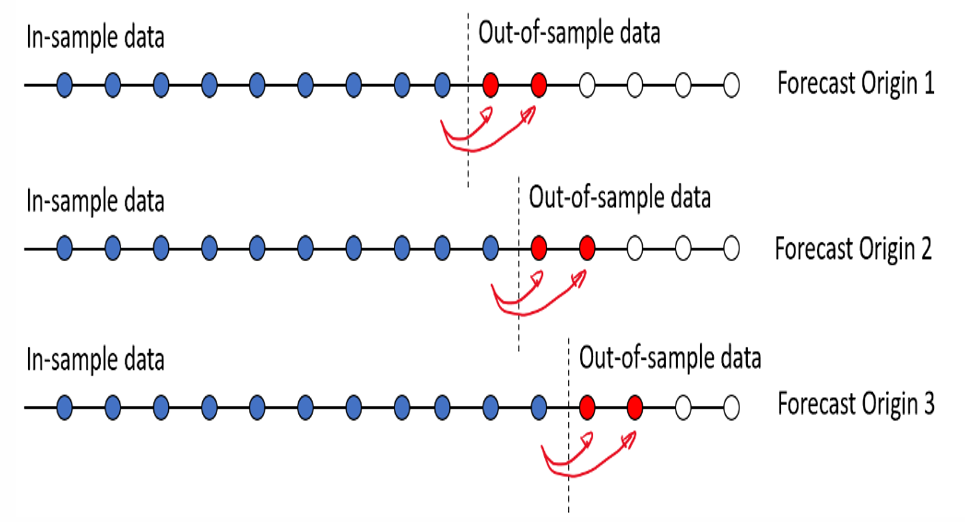
\includegraphics[width=0.95\paperwidth]{../static/course_3_img/in_sample_out_sample.PNG}}  
\end{frame}

\begin{frame}
  \frametitle{Underfit, Optimal, Overfit}
     \makebox[\linewidth]{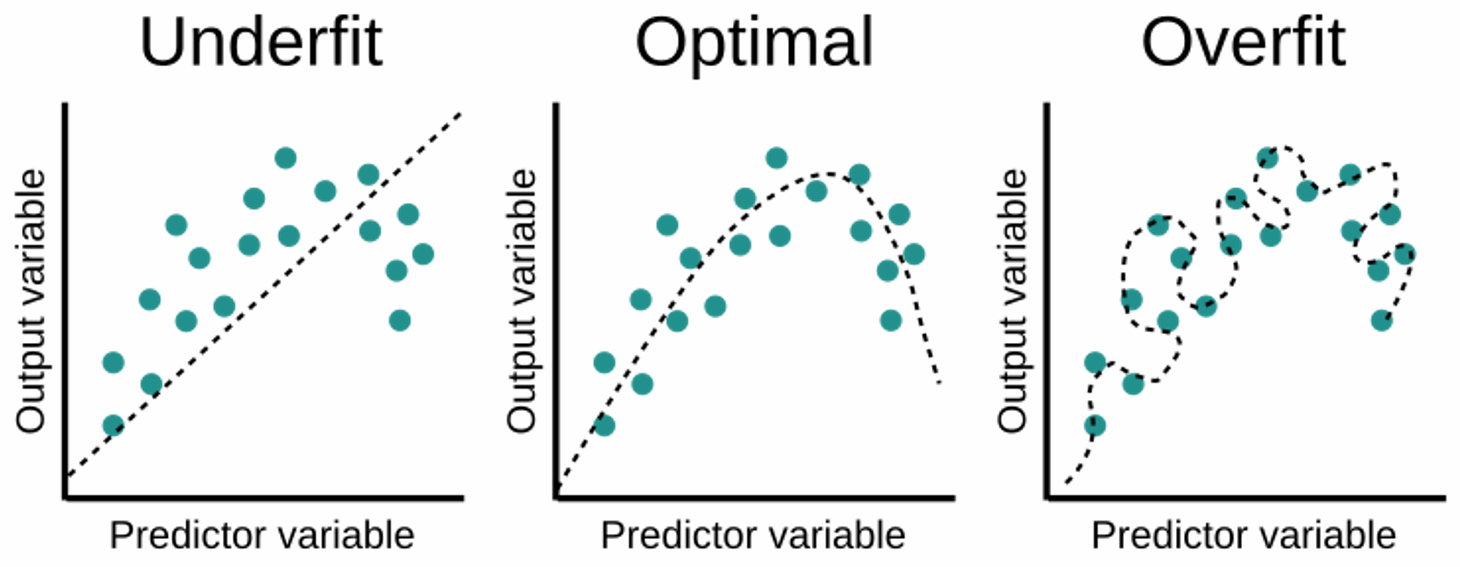
\includegraphics[width=0.95\paperwidth]{../static/course_3_img/overfit_underfit.PNG}}  
\end{frame}

\begin{frame}{Forecast Errors}

  \begin{block}{Definition: Forecast Errors}
    A forecast error is the difference between an observed value and its forecast

    \begin{equation*}
      e_{T+h} = y_{T+h} - \hat{y}_{T+h}|Y_T, \dots, Y_1
    \end{equation*}
  \end{block}

\medskip
  
\begin{wideitemize}
    \item The conditional set $Y_T, \dots, Y_1$ should only be taken from the training dataset
    \item The true value $y_{T+h}$ is taken from the test set
    \item Unlike residuals, forecast errors on the test involve multi-step forecasts
    \item These are the \textbf{true} forecast error, as the test data is not used to compute $\hat{y}_{T+h}$
  \end{wideitemize}
  
\end{frame}

\begin{frame}
  \frametitle{Example: Forecasting Beer Production}
     \makebox[\linewidth]{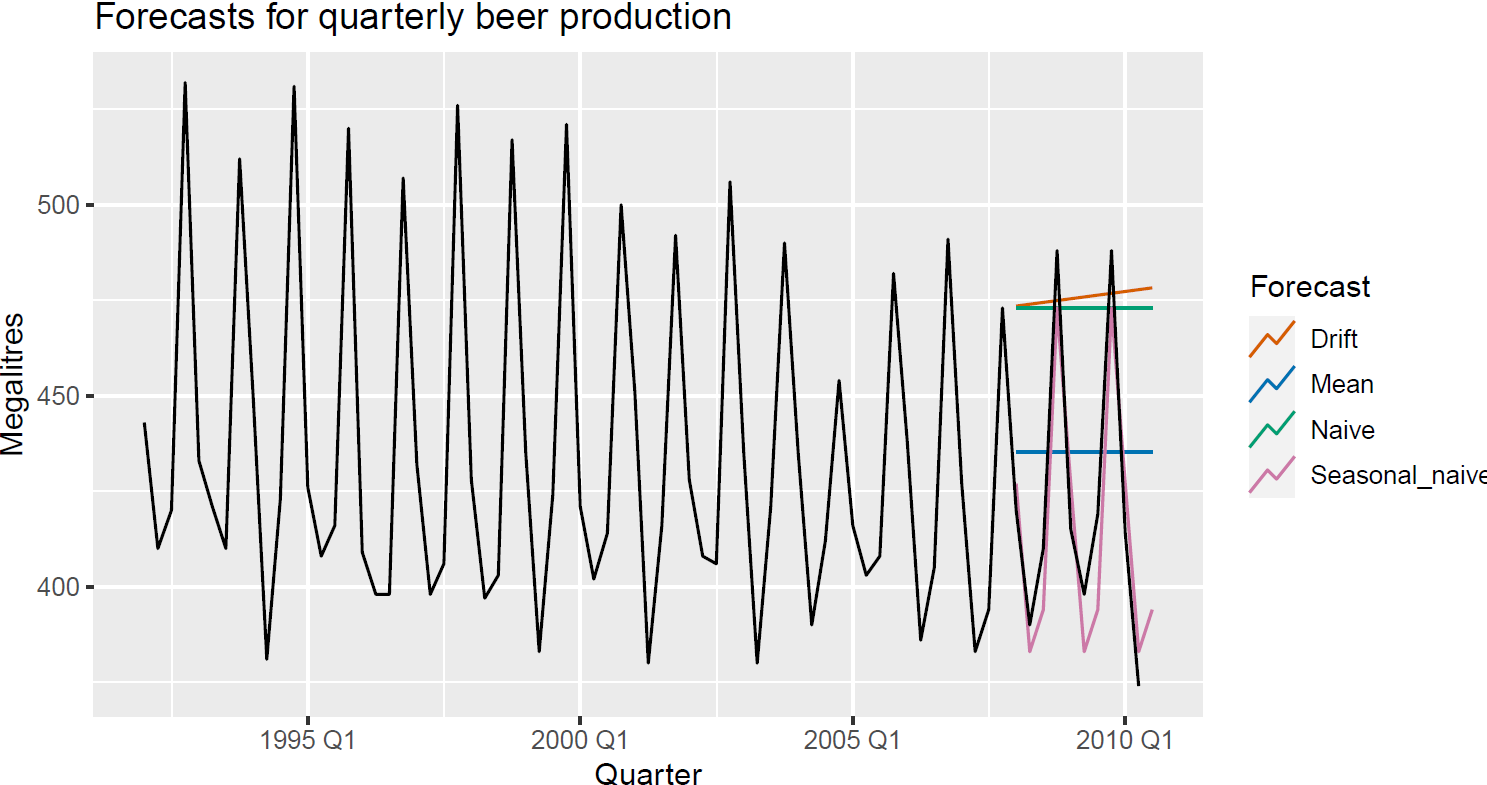
\includegraphics[width=0.95\paperwidth]{../static/course_3_img/beer_forecast.PNG}}  
\end{frame}

\begin{frame}{Measures of Forecast Accuracy}

  \begin{alertblock}{Main Metrics}
    \begin{wideitemize}
    \item \textbf{MAE}: mean absolute errors $\frac{1}{S}\sum_{s \in S} |e_{s, T+h}|$
    \item \textbf{MSE}: mean squared errors $\frac{1}{S}\sum_{s \in S} (e_{s, T+h})^2$
    \item \textbf{MAPE}: mean absolute percentage errors $\frac{1}{S}100*\sum_{s \in S} \frac{|e_{s, T+h}|}{|y_{s, t+h}|}$
    \item \textbf{RMSE}: root mean squared errors: $\sqrt{\frac{1}{S}\sum_{s \in S} (e_{s, T+h})^2}$
    \end{wideitemize}
  \end{alertblock}

  With:\\
  
  \begin{itemize}
  \item $y_{T+h}$: T+h observation, h being the horizon (h = 1, 2, ..., H)
  \item $\hat{y}_{T+h|T}$: the forecast based on data up to time $T$
  \item $e_{T+h} = y_{T+h} - \hat{y}_{T+h|T}$: The forecast errors
  \item $S$ is the testing sample
  \end{itemize}
\end{frame}

\begin{frame}{Scaling}  
  \begin{wideitemize}
  \item MAE, MSE and RMSE are all \textbf{scale dependent}
  \item MAPE is scale independent but is only sensible if $y_t >> 0 \qquad \forall \ t$
  \item \textbf{Most commonly used: Time Cross-Validation with the lowest RMSE}
  \end{wideitemize}  
\end{frame}


\begin{frame}
  \frametitle{Time Series Cross-Validation}
     \makebox[\linewidth]{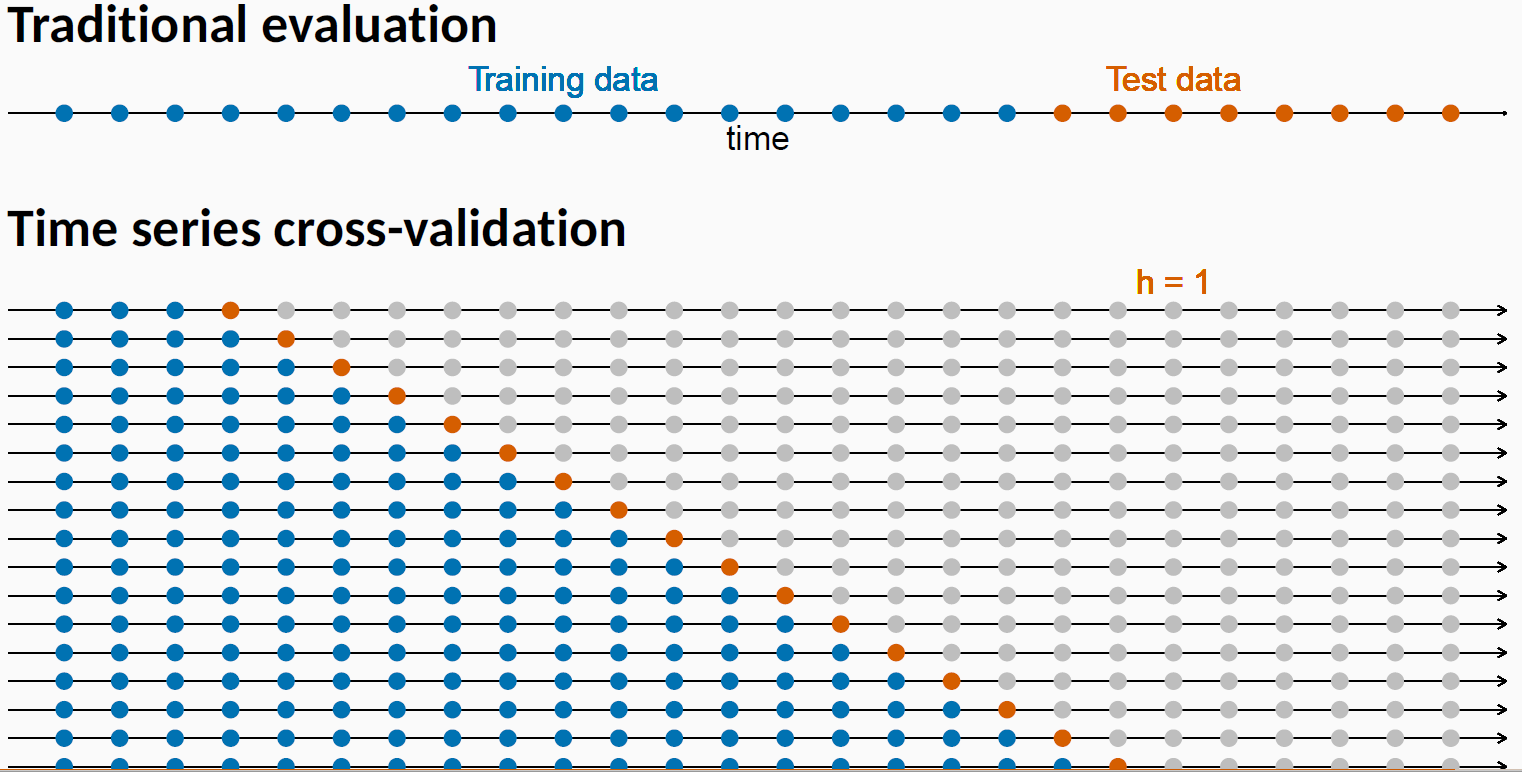
\includegraphics[width=0.95\paperwidth]{../static/course_3_img/time_series_cv_1.PNG}}  
  \end{frame}

\begin{frame}
  \frametitle{Time Series Cross-Validation}
     \makebox[\linewidth]{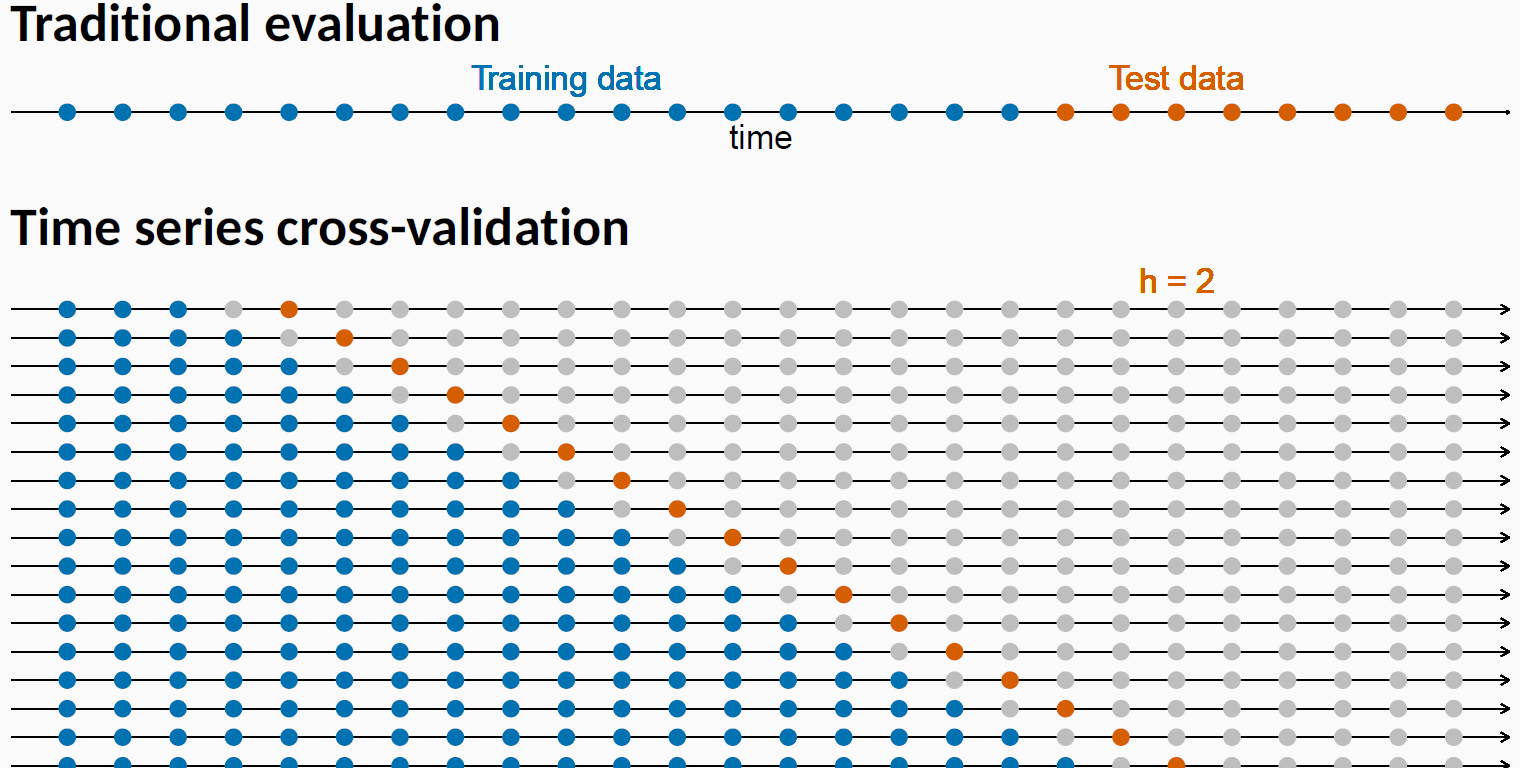
\includegraphics[width=0.95\paperwidth]{../static/course_3_img/time_series_cv_2.PNG}}  
  \end{frame}

\begin{frame}
  \frametitle{Time Series Cross-Validation}
     \makebox[\linewidth]{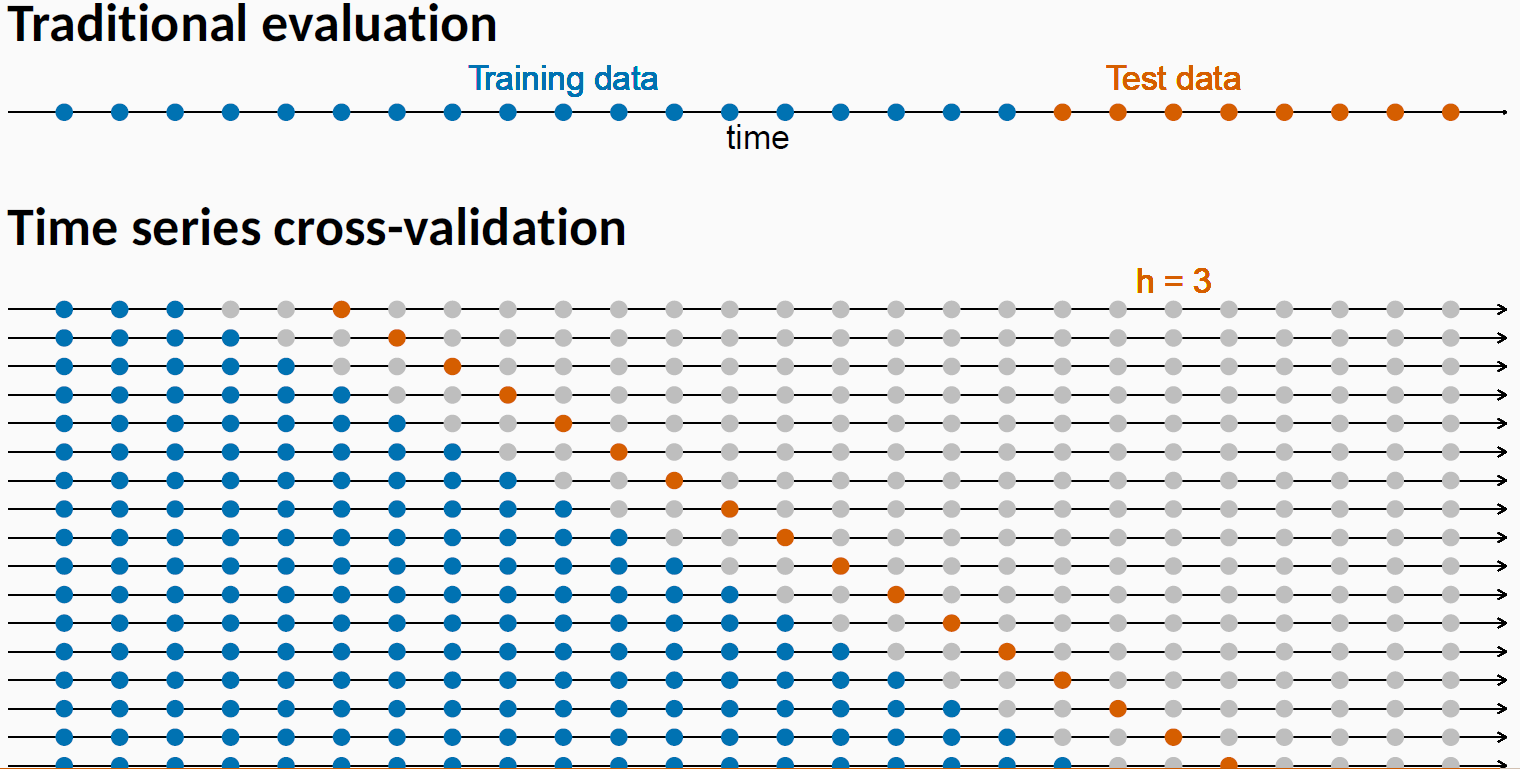
\includegraphics[width=0.95\paperwidth]{../static/course_3_img/time_series_cv_3.PNG}}  
  \end{frame}

\begin{frame}
  \frametitle{Time Series Cross-Validation}
     \makebox[\linewidth]{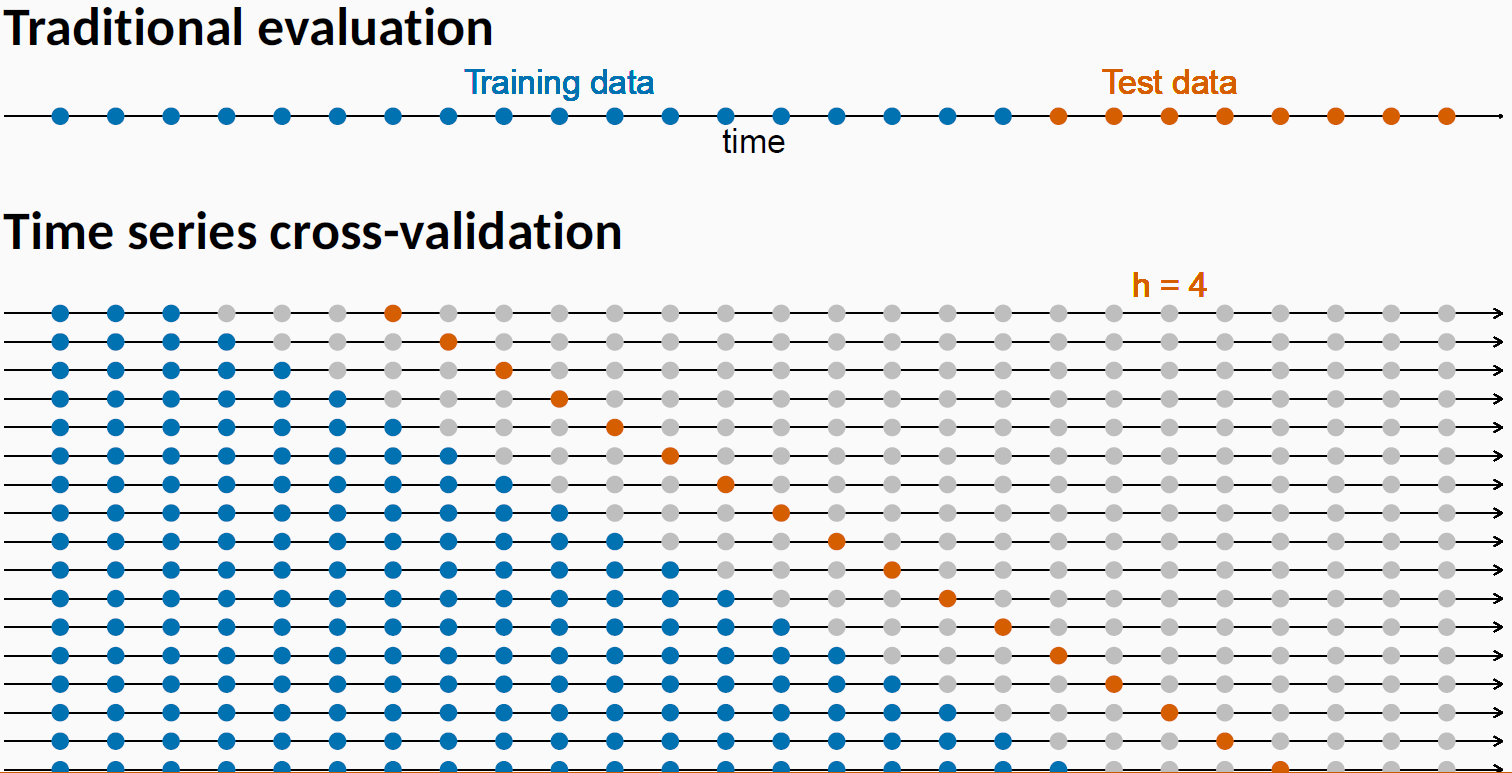
\includegraphics[width=0.95\paperwidth]{../static/course_3_img/time_series_cv_4.PNG}}  
  \end{frame}

\begin{frame}
  \frametitle{Time Series Cross-Validation}
     \makebox[\linewidth]{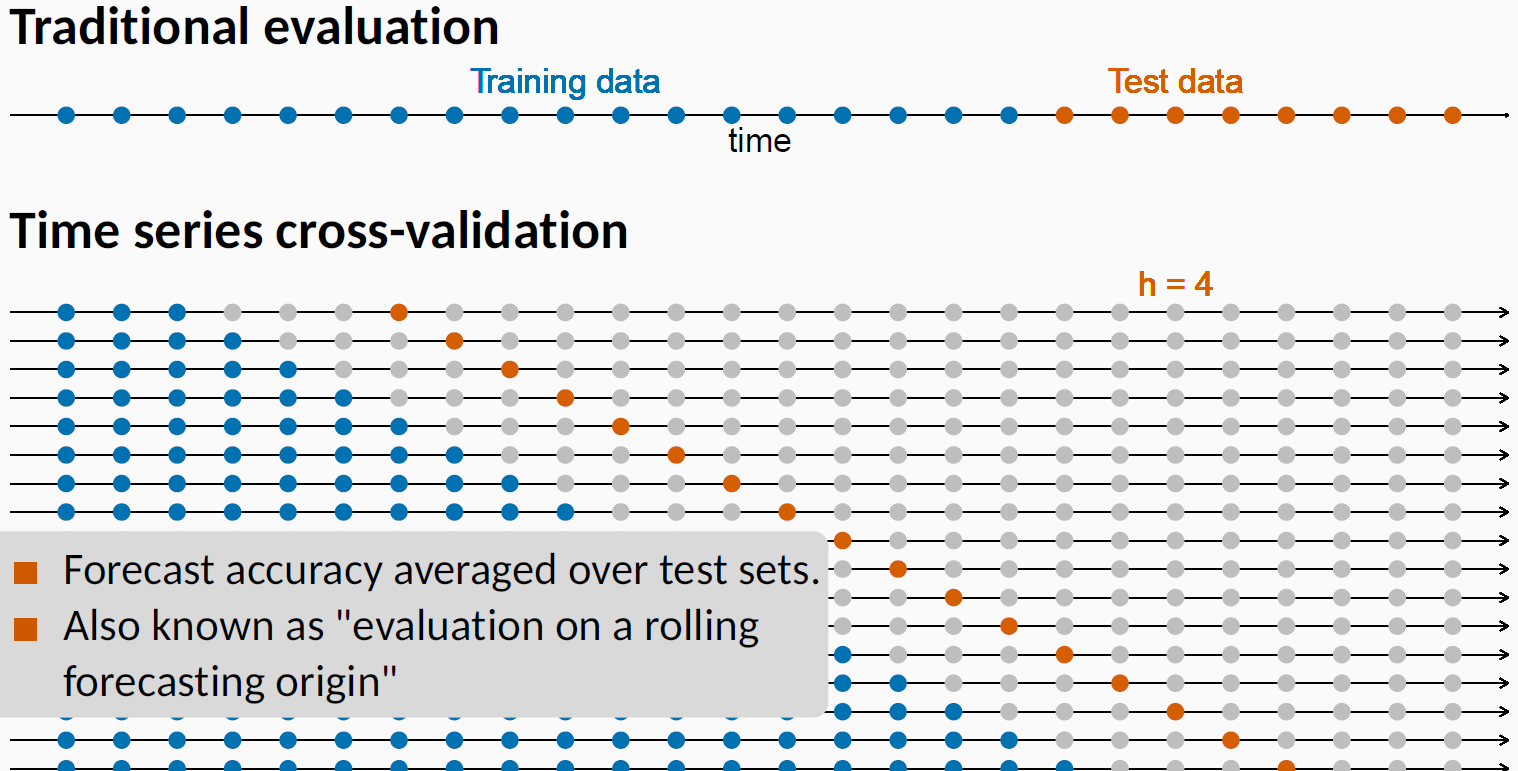
\includegraphics[width=0.95\paperwidth]{../static/course_3_img/time_series_cv_5.PNG}}  
  \end{frame}


    \begin{frame}
      \frametitle{Framework RMSE Output}
  \makebox[\linewidth]{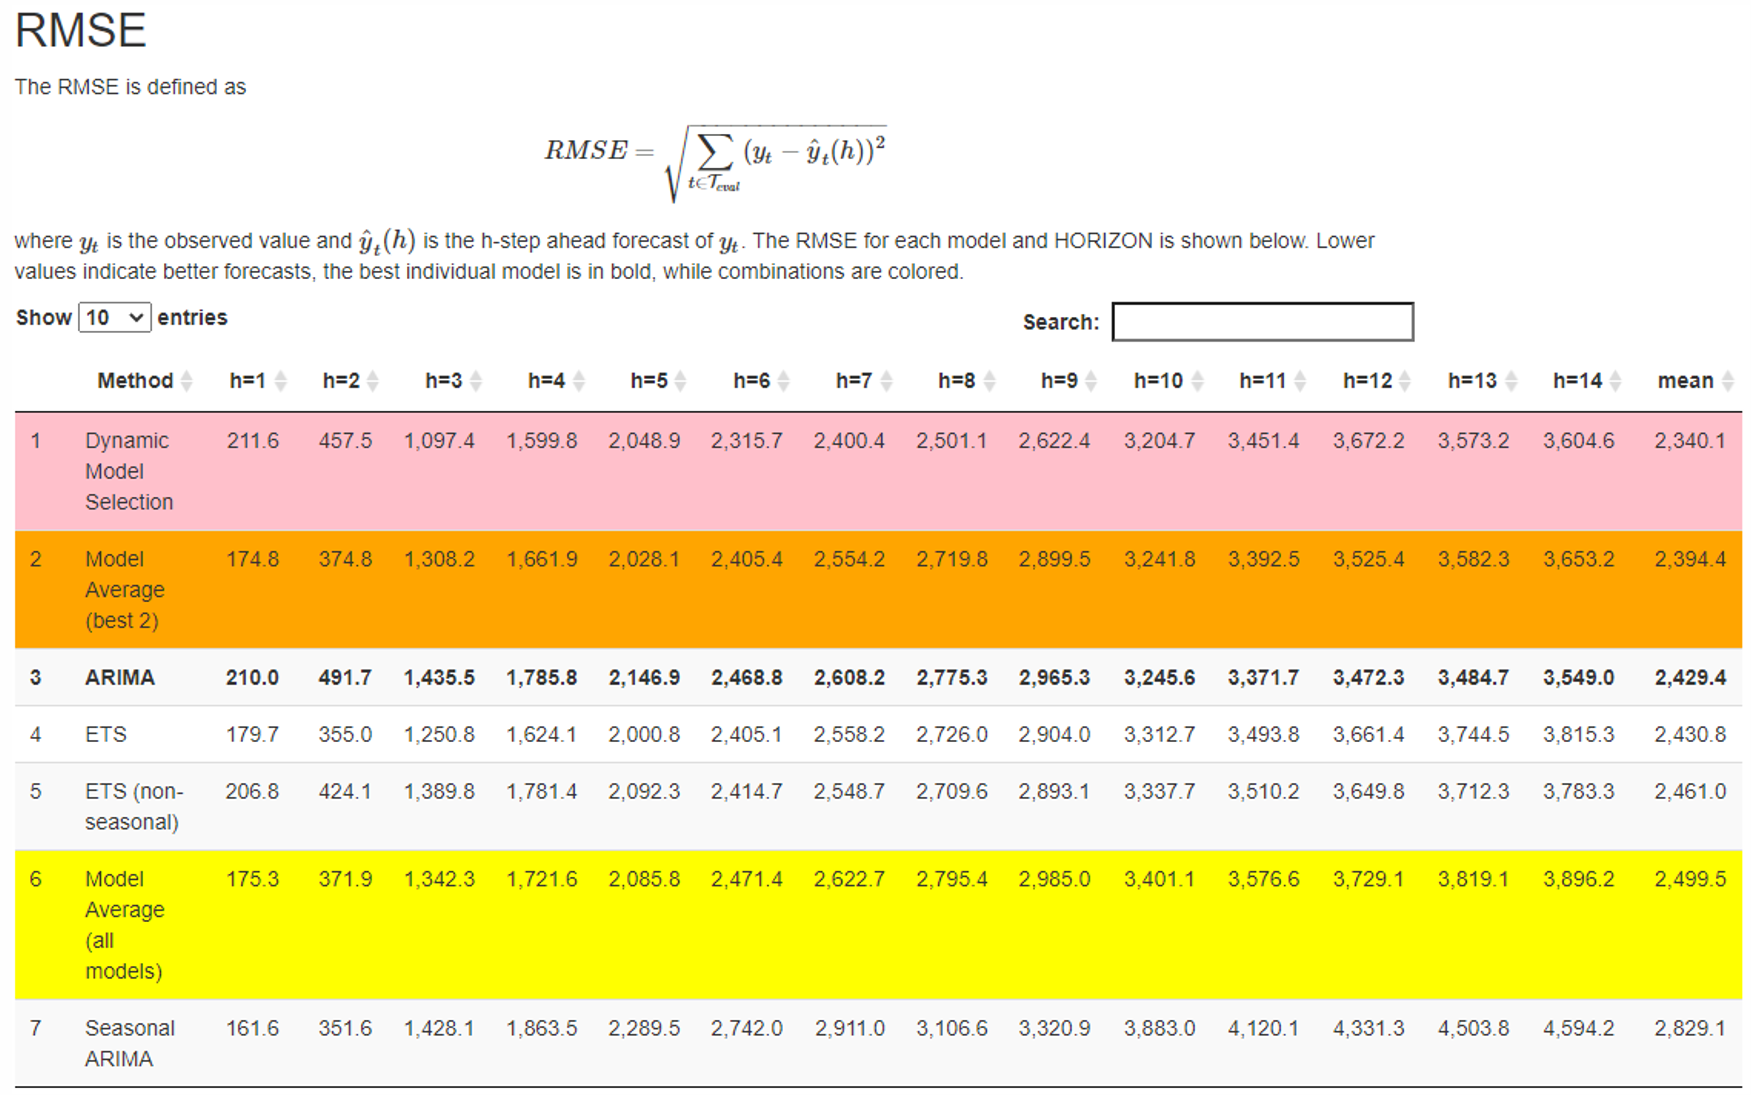
\includegraphics[width=0.85\paperwidth]{../static/course_3_img/rmse_output.PNG}}
  \hspace*{15pt}\hbox{\scriptsize Credit:\thinspace{\scriptsize\itshape IMF Framework}}      
    \end{frame}


    \begin{frame}
      \frametitle{Nemenyi Test}

      \begin{wideitemize}
        \item We can rank the model by RMSE (or another metric), but are the RMSE significantly different? 
        \item Maybe Model 1 can have a lower RMSE than Model 2, but the difference in RMSE is non-significant
        \item In which case, we could pool the two models together
        \item Use a non-parametric test to test the hypothesis of equal RMSE, with the test statistic:
          \begin{equation*}
            r_{\alpha, K, N} \approx \frac{q_{\alpha, K}}{\sqrt{2}} \sqrt{\frac{K (K+1)}{6N}}
          \end{equation*}
      \end{wideitemize}      
    \end{frame}

    \begin{frame}
      \frametitle{Nemenyi Test in Practice}
  \makebox[\linewidth]{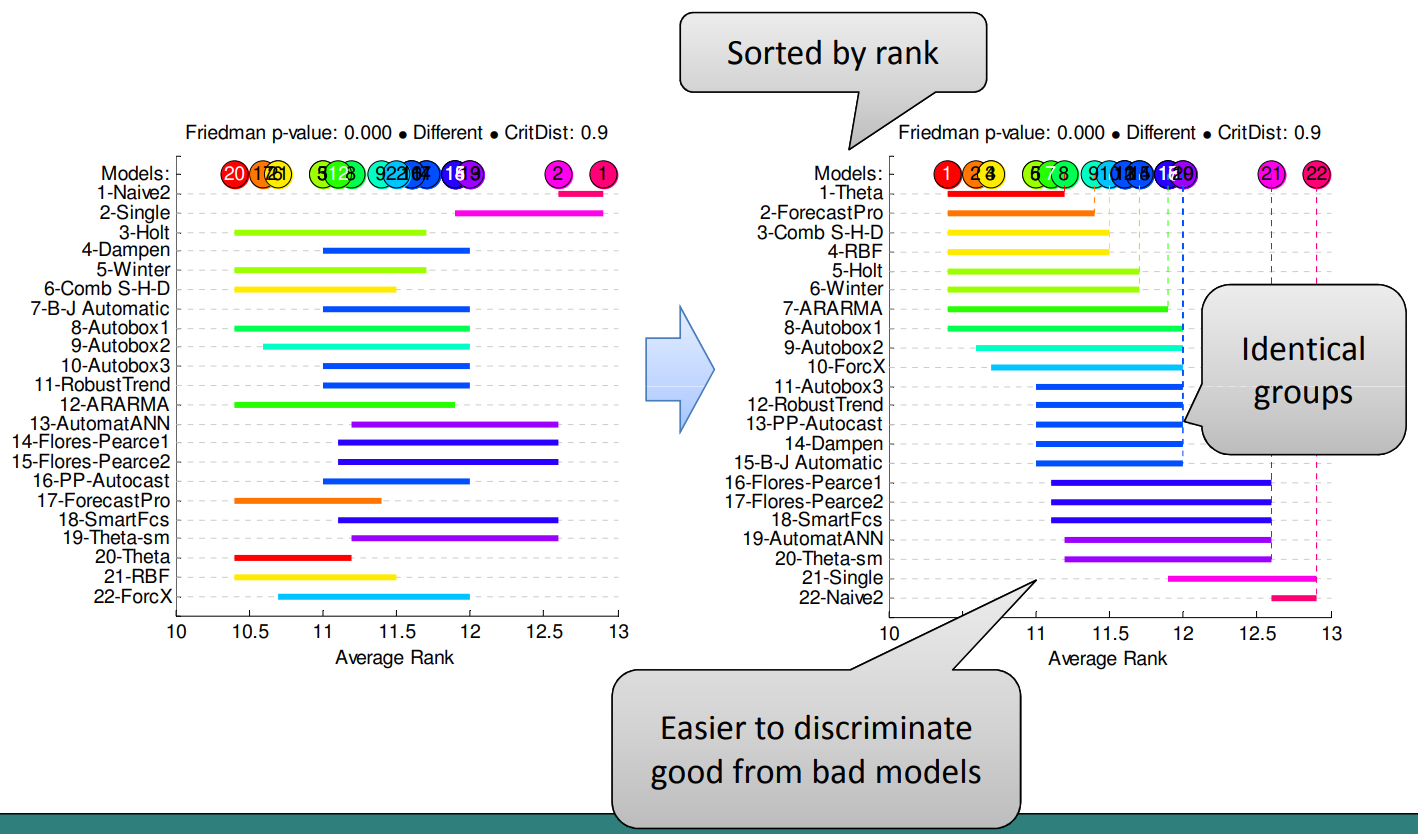
\includegraphics[width=0.85\paperwidth]{../static/course_3_img/nemenyi_test.PNG}}
  \hspace*{15pt}\hbox{\scriptsize Credit:\thinspace{\scriptsize\itshape Nikolaos Kourentzes}}      
    \end{frame}

    
    
\section{Model Combination and Selection}

\begin{frame}
  \frametitle{Combination of Models}

  \begin{wideitemize}
    \item Combining model provides a more reliable forecast, overcoming the risk of relying on a single model
    \item Estimate all the models, determine the cross-validated errors
    \item Define a pool of "good" models and reject the other models, based on their out of sample performance. Define a \textbf{rejection threshold} to determine the "bad" models, based on the distribution of the RMSE
      \begin{equation*}
        \text{Threshold} = Q(0.75) + 1.5*\text{IQR}
      \end{equation*}
      \begin{itemize}
      \item Where $Q(0.75)$ is the 75th quantile of the RMSE distribution and IQR the interquantile range ($Q(0.75) - Q(0.25)$)
      \end{itemize}
    \item Then, weight each forecast of the eligible model by the relative performance of their model, the best models having the highest weight
    \item Advantage: optimize performance and reduce modeling risks, doesn’t rely on a single model: model diversity is advantageous    
  \end{wideitemize}
  
\end{frame}

\begin{frame}
  \frametitle{Dynamic Model Selection: Principles}

  \begin{wideitemize}
    \item Some models are better for modelling long-term dynamics, while others are better are short-term dynamics 
    \item Time-varying volatility matters. As volatility increases, models focusing on the short term have an advantage
    \item Dynamically account for changes in the behaviour of the time series:
      \begin{itemize}
      \item Combining high performing forecasts
      \item Selecting a well performing forecast based on local performance
      \end{itemize}
  \end{wideitemize}  
\end{frame}


\begin{frame}
  \frametitle{Dynamic Model Selection: Implementation}

  \begin{wideitemize}
  \item \textbf{Combining high-performance forecasts:}
    \begin{itemize}
    \item Compute unweighted average of forecasts. Although it seems better to estimate “optimal” weights, weights estimation introduces additional uncertainty  
    \end{itemize}
  \item Selecting a well performing forecast based on \textbf{recent performance}
    \begin{itemize}
    \item \textbf{Rolling performance of the previous week} to select the forecast for the next origin. 
    \end{itemize}
    
  \item Consider ETStrig, ARIMAtrig, ARIMA stoch, and TBATS comp. All these models capture information differently
    \begin{itemize}
    \item \textbf{Model diversity is advantageous} both for selection and combination between forecasts
    \end{itemize}
  \end{wideitemize}  
\end{frame}

 \begin{frame}
 \frametitle{Out-of-Sample Performances via Rolling Origins}
  \makebox[\linewidth]{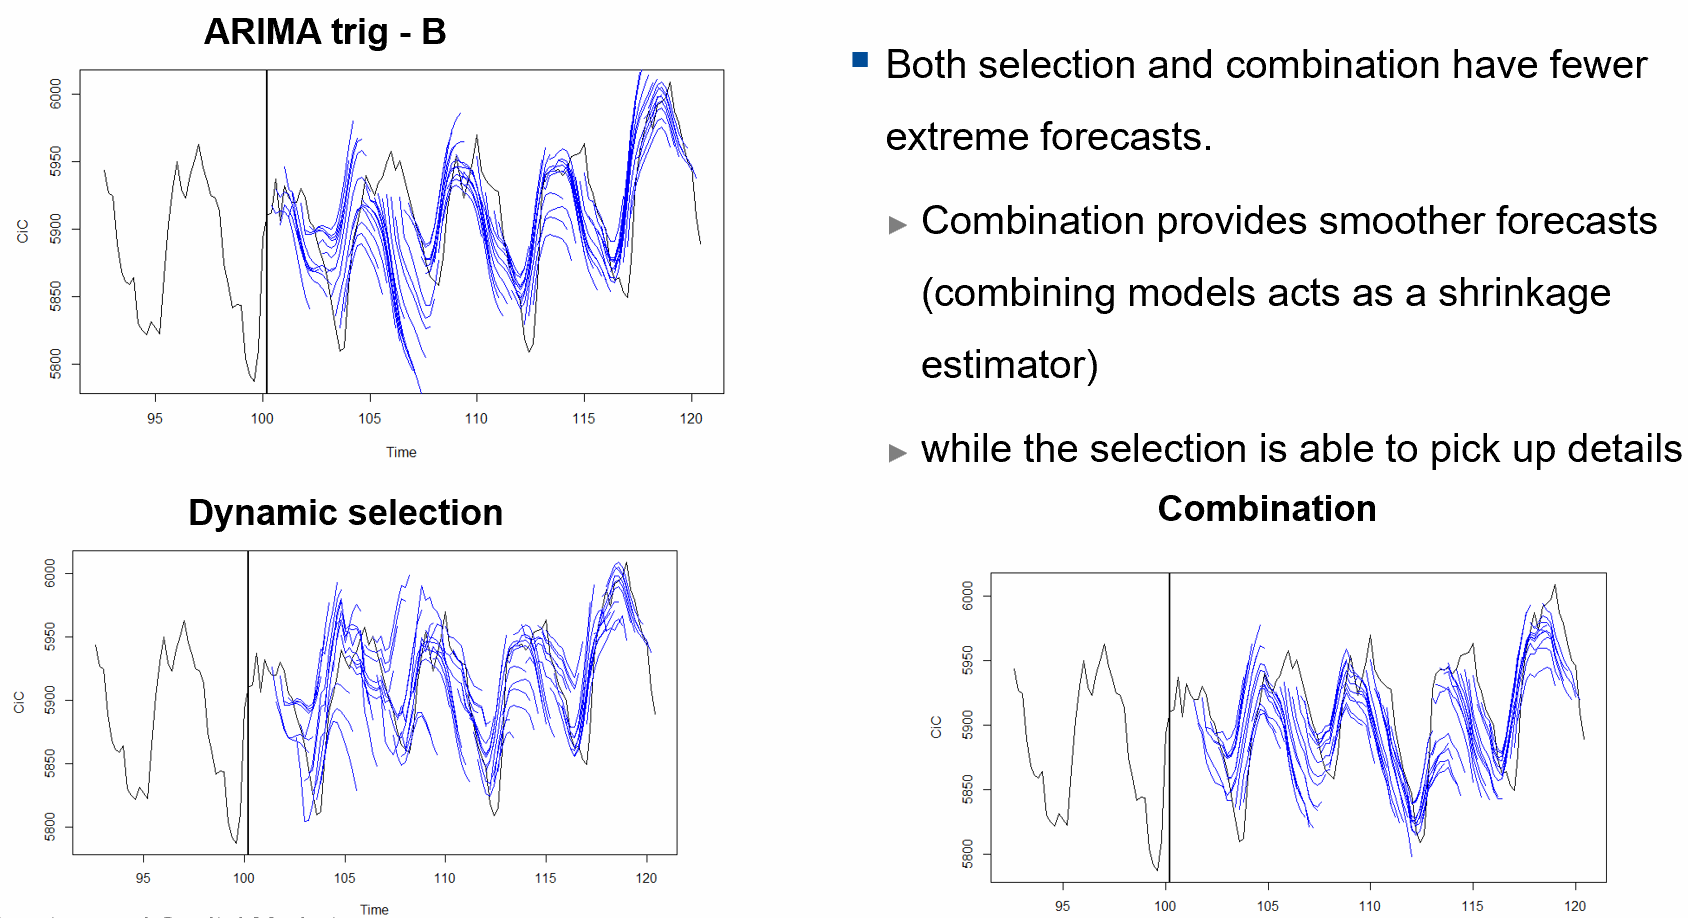
\includegraphics[width=0.75\paperwidth]{../static/course_3_img/arima_combination_selection.PNG}}
  \hspace*{15pt}\hbox{\scriptsize Credit:\thinspace{\scriptsize\itshape Author}}      
 \end{frame}


\section{Forecasts Reconciliation}
\begin{frame}
  \frametitle{Forecasts Reconciliation of the Autonomous Factors}

  Forecast the autonomous factors using a hierarchical modeling approach, with different models for each autonomous factor:\\
  \medskip

  \begin{wideitemize}
  \item Forecasting the sum of the autonomous factors separately\\
  \item Reconciling the forecasts using aggregation technics as described for instance in Hyndman, Rob J., et al. "Optimal combination forecasts for hierarchical time series." (2011)
  
  \item Use either OLS  or the “minT” approach: minimize the trace of the VarCov forecast matrix. Exploit the covariance among regressors to maximize the accuracy of the hierarchical forecasts    
  \end{wideitemize}   
\end{frame}

 \begin{frame}
 \frametitle{Reconciliation via Hierarchical Forecasts}
  \makebox[\linewidth]{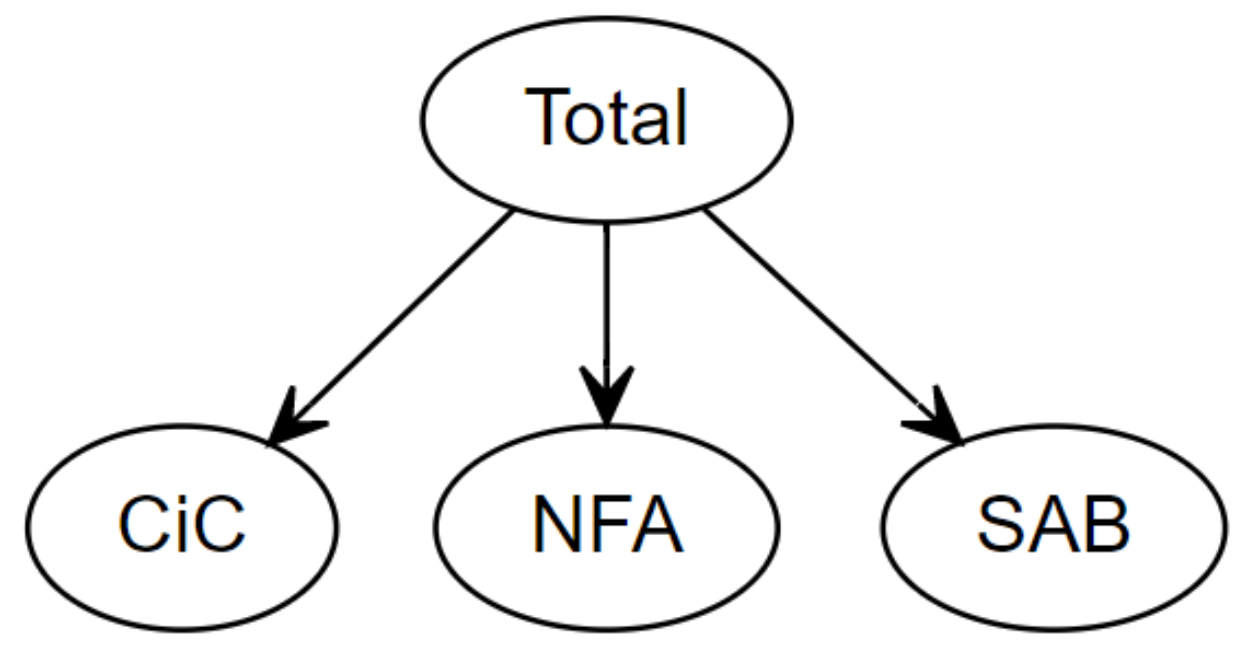
\includegraphics[width=0.75\paperwidth]{../static/course_3_img/hierarchical_forecasts.PNG}}
  \hspace*{15pt}\hbox{\scriptsize Credit:\thinspace{\scriptsize\itshape Author}}      
 \end{frame}


 \begin{frame}
 \frametitle{General Approach}

  \makebox[\linewidth]{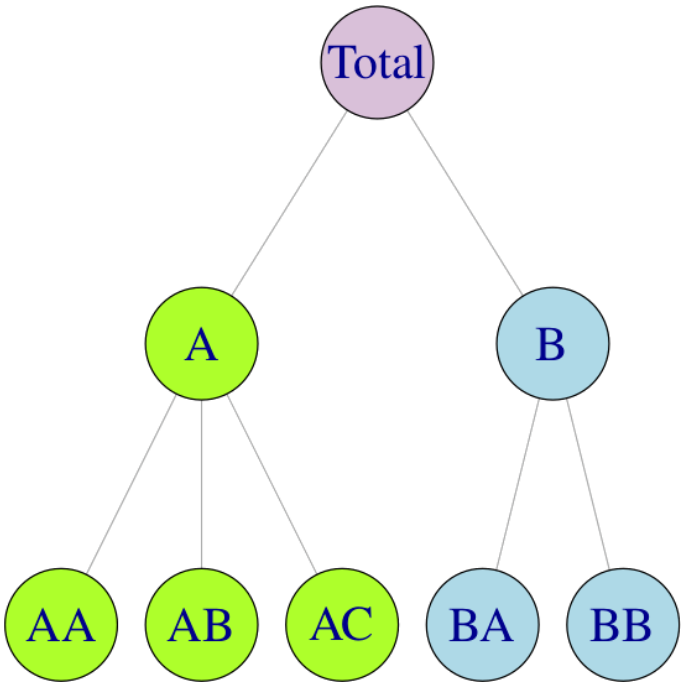
\includegraphics[width=0.5\paperwidth]{../static/course_3_img/hierarchical_forecasts_two_levels.PNG}}
  \hspace*{15pt}\hbox{\scriptsize Credit:\thinspace{\scriptsize\itshape https://otexts.com/fpp3/reconciliation.html}}      
 
 \end{frame}


 \begin{frame}
 \frametitle{Formalization}

 \begin{wideitemize}
 \item We can express the total (top level, $y_t$) via a summing matrix $S$ of the low level elements $y^L_t$
   \begin{equation*}
     y_t = S y^L_t
   \end{equation*}
 \item Then, we can express the whole system via a grouping matrix summing all the individual elements (also called base forecast $y^b_t$), so have a consistent approach irrespective of the level structure
   \begin{equation*}
     \tilde{y_t} = S*G*y^b_{h}
   \end{equation*}
 \end{wideitemize}

 \makebox[\linewidth]{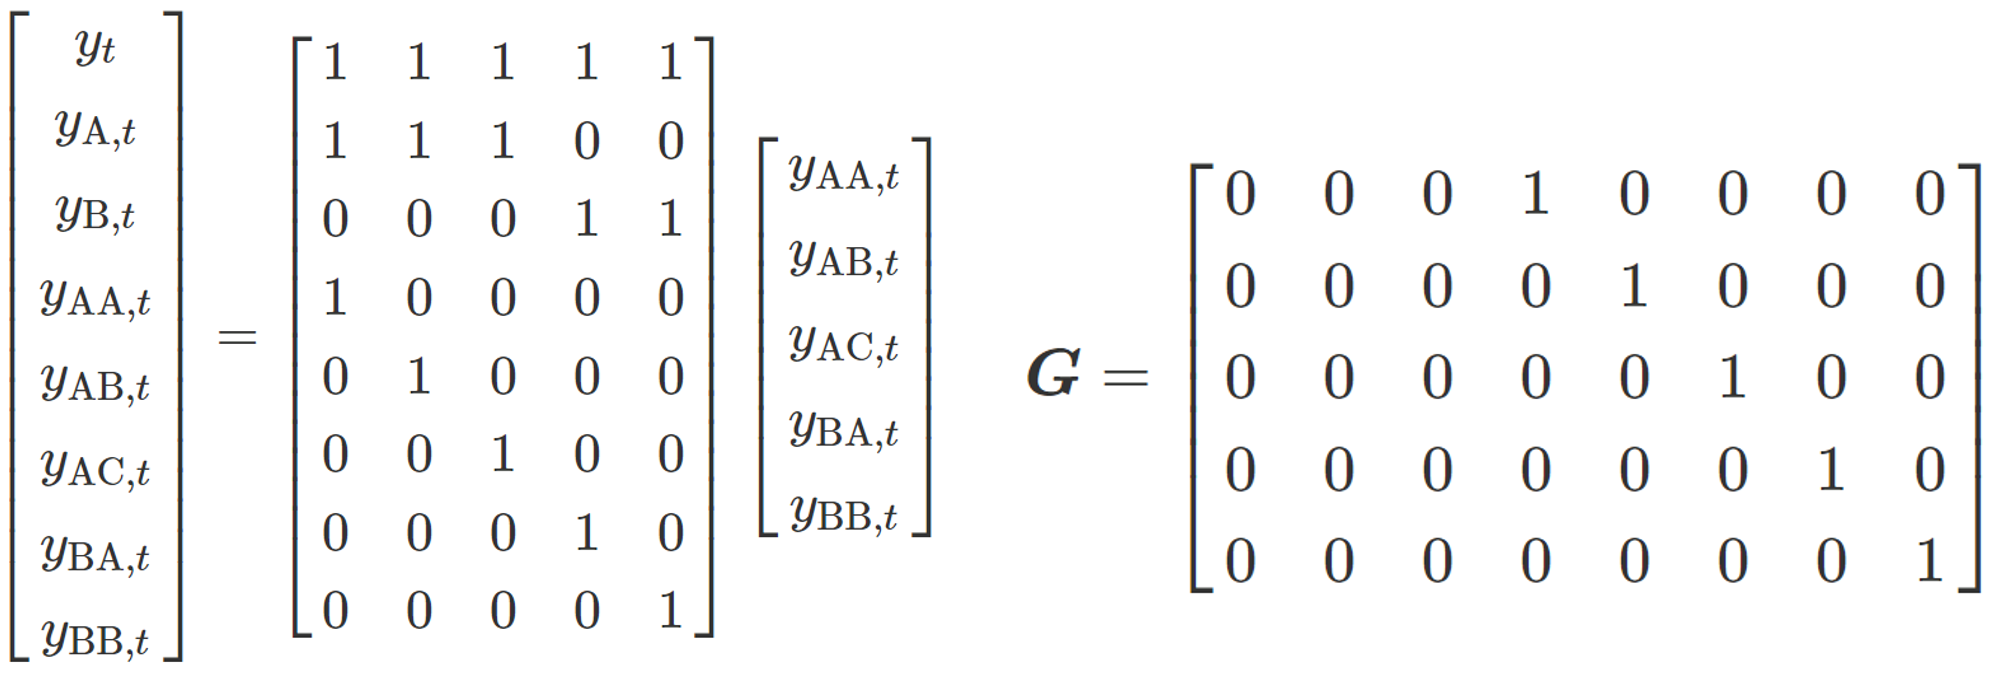
\includegraphics[height=0.25\paperheight]{../static/course_3_img/hierarchical_forecasts_two_matrices.PNG}}
 \hspace*{15pt}\hbox{\scriptsize Credit:\thinspace{\scriptsize\itshape otexts.com/fpp3/reconciliation.html}}      
 
 \end{frame}


 \begin{frame}
   \frametitle{The Min Trace Approach}
   \begin{block}{Forecasts Errors in a Hierarchical System}
     \begin{equation*}
       V_h = \mathbb{V}[y_{T+h} - \tilde{y_h}] = SGW_hG'S'
     \end{equation*}
   where $W_h = \mathbb{V}[y_{T+h} - \tilde{y^b_h}]$ the variance-covariance matrix of the base vector
 \end{block}
\bigskip

\begin{itemize}
  \item The objective is to find a matrix $G$ to minimize the variance-covariance matrix of the corresponding base forecast errors
  \item Because the error variances are on the diagonal of $V_h$, minimizing the forecasting errors is equivalent to minimizing the trace of $V_h$
  \item Wickramasuriya et al. (2019) show that the minimized trace matrix is given by:
    \begin{equation*}
      G = (S'W^{-1}_hS)^{-1}S'W_h^{-1}
    \end{equation*}
  \item This approach is called the \textbf{MinT (or Minimum Trace) optimal reconciliation approach}
    
\end{itemize} 
\end{frame}

\end{document}